\documentclass[%
%draft,
11pt,%
twoside,%
titlepage,%
swissgerman,%
headsepline%
]{scrartcl}

\usepackage{lastpage}
\usepackage{amsthm}
\usepackage{amssymb}
\usepackage{geometry}
\usepackage{graphicx}
\usepackage[dvipsnames]{xcolor}
\usepackage[utf8]{inputenc}
\usepackage[swissgerman]{babel}
\usepackage{lscape}
\usepackage[framemethod=TikZ]{mdframed}
\usepackage[most]{tcolorbox}
\usepackage{enumerate}
\usepackage{units}
\usepackage{nicefrac}
\usepackage{pgf,tikz}
\usepackage{tikz-3dplot}
\usepackage{tkz-euclide}
\usetikzlibrary{arrows}
\usetikzlibrary{arrows.meta}
\usetikzlibrary{patterns}
\usetikzlibrary{positioning}
\usetikzlibrary{shadows}
\usetikzlibrary{quotes, angles}
\usepackage{colortbl}
\usepackage{hhline}
\usepackage{multirow}
\usepackage[extendedchars]{grffile}
\usepackage{caption}
\usepackage{multicol,calc}
\usepackage{blindtext}
\usepackage{pdfpages}
\usepackage{hyperref}
\usepackage{framed}

\usepackage{marginnote}
\usepackage{qrcode}
<<<<<<< Updated upstream
\qrset{height=9ex}
=======
\qrset{height=7ex}
>>>>>>> Stashed changes

\usepackage{longtable}
\usepackage{listings}
\usepackage{wrapfig}

\usepackage{fontawesome} % Oder FontAwesome, falls du ein Augensymbol aus einer
\newcommand{\faEyeLightGray}{\textcolor{lightgray}{\faEye}} % Custom command for the gray eye icon
\newcommand{\faReturnGray}{\textcolor{gray}{\faMailReply}} % Custom command for the gray eye icon
\usepackage{pifont} % weitere Zeichen

% package für plots mit dem Befehl axes
\usepackage{pgfplots}



% Command, um Tabellen-Spalten anzupassen
\newcommand{\spaltenheight}{\rule{0mm}{3ex}}
\newcommand{\spaltenwidth}{\rule{3cm}{0mm}}
\newcommand{\spaltensep}{\\[1ex]}
%\arrayrulecolor{darkgreen}
\doublerulesepcolor{white}

% colors
\definecolor{lightyellow}{rgb}{1,1,0.8}
\definecolor{Gray}{gray}{0.9}
\definecolor{lightgray}{rgb}{0.7, 0.7, 0.7}
\definecolor{darkblue}{rgb}{0,0,0.55}
\definecolor{firebrick}{rgb}{0.7,0.13,0.13}
\definecolor{seagreen}{rgb}{0.18,0.55,0.34}
\definecolor{emerald}{HTML}{50C878} % color of Definition
\definecolor{whitesmoke}{HTML}{F5F5F5} % background for environments
\definecolor{myblizzardblue}{HTML}{87CEEB} % color of Satz

% Für Definitionen im Fliesstext
\newcommand{\definition}[1]{\colorbox{emerald}{#1}}
% Für Regeln im Fliesstext
\newcommand{\regel}[1]{\colorbox{myblizzardblue}{#1}}
% Für Merke/Achtungs im Fliesstext
\newcommand{\merke}[1]{\colorbox{firebrick}{#1}}
% Geogebra-Link
\newcommand{\geogebralink}{\href{https://www.geogebra.org/calculator}{\texttt{geogebra.org}}}

% Umgebungen
\theoremstyle{definition}
    \newtheorem{bsp}{Beispiel}[subsection] % Beispiele
    \newtheorem{bem}{Bemerkung}[subsection] % Bemerkungen
\theoremstyle{plain}
    \newtheorem{thm}{Theorem} % Theorem [subsection]
    \newtheorem{satz}{Satz} % Satz [subsection]

% Umgebung lsg mit dynamischer Referenzierung und Label
\newcommand{\concatueb}[1]{ueb:#1}% Definition für concatueb
\newcommand{\concatlsg}[1]{lsg:#1}% Definition für concatlsg

\newcounter{uebcounter}[section]
\renewcommand{\theuebcounter}{\thesection.\arabic{uebcounter}}  % Zählerformat: Abschnitt.Übung

\newenvironment{lsg}[1]{%
<<<<<<< Updated upstream
    \par\noindent\textbf{Notizen zu Übung \theuebcounter\label{\concatlsg{#1}}}
=======
    \par\noindent\textbf{Notizen zu Übung \ref{\concatueb{#1}}}\label{\concatlsg{#1}}
>>>>>>> Stashed changes
    \hfill\hyperref[\concatueb{#1}]{\faReturnGray}\par % Hyperref-Button zurück zur Übung
}{%
    \par%
}

\newenvironment{uebenv}[1]{%
    \refstepcounter{uebcounter}
    \par\noindent\textbf{Übung \theuebcounter.}%
    \label{\concatueb{#1}}\hfill\hyperref[\concatlsg{#1}]{\faEyeLightGray}\par
}{%
    \par
}

% Umgebung für Definitionen
\newcounter{deff}[section]\setcounter{deff}{0}
\renewcommand{\thedeff}{\arabic{section}.\arabic{deff}}

\newenvironment{cdef}[1][]{%
    \refstepcounter{deff} 
    \ifstrempty{#1}%
    % if condition (without title)
    {\mdfsetup{%
        frametitle={%
            \tikz[baseline=(current bounding box.east),outer sep=0pt]
            \node[anchor=east,rectangle,fill=emerald]
            {\strut Definition~\thedeff};}
        }%
    % else condition (with title)
    }{\mdfsetup{%
        frametitle={%
            \tikz[baseline=(current bounding box.east),outer sep=0pt]
            \node[anchor=east,rectangle,fill=emerald]
            {\strut Definition~\thedeff:~#1};}%
        }%
    }%
% for both conditions
    \mdfsetup{%
        innertopmargin=10pt,linecolor=emerald,%
        backgroundcolor=whitesmoke,%
        linewidth=2pt,topline=true,%
        frametitleaboveskip=\dimexpr-\ht\strutbox\relax%
    } 
\begin{mdframed}[]\relax}{%
\end{mdframed}}

% Farbig umrahmte Umgebung Satz
\newcounter{satzz}[section]\setcounter{satzz}{0}
\renewcommand{\thesatz}{\arabic{section}.\arabic{satzz}}

\newenvironment{csatz}[1][]{%
    \refstepcounter{satzz}
 
    \ifstrempty{#1}%
    % if condition (without title)
    {\mdfsetup{%
        frametitle={%
            \tikz[baseline=(current bounding box.east),outer sep=0pt]
            \node[anchor=east,rectangle,fill=myblizzardblue]
            {\strut Satz~\thesatz};}
        }%
    % else condition (with title)
    }{\mdfsetup{%
        frametitle={%
            \tikz[baseline=(current bounding box.east),outer sep=0pt]
            \node[anchor=east,rectangle,fill=myblizzardblue]
            {\strut Satz~\thesatz:~#1};}%
        }%
    }%
% for both conditions
    \mdfsetup{%
        innertopmargin=10pt,linecolor=myblizzardblue,%
        backgroundcolor=whitesmoke,%
        linewidth=2pt,topline=true,%
        frametitleaboveskip=\dimexpr-\ht\strutbox\relax%
    }
\begin{mdframed}[]\relax}{%
\end{mdframed}}

% kein Einzug bei neuem Abschnitt
\setlength{\parindent}{0pt} \setlength{\parskip}{1em}
\pagestyle{headings} % gemachte Einstellungen anwenden


<<<<<<< Updated upstream
=======

>>>>>>> Stashed changes
\subject{\includegraphics[width=0.618\textwidth]{pictures/ejost}}
\title{Folgen \& Reihen}
\subtitle{Look up the Number!}
\author{}
\date{}
\lowertitleback{
\includegraphics[height=1cm]{pictures/gymfmslerbermattlogo.eps}
\hfill%\copyright%
{\begin{tikzpicture}
  % Draw the rounded rectangle and clip the image to it
  \clip [rounded corners=5mm] (0,0) rectangle (1,1); % Adjust dimensions as needed
  \node at (0.5,0.5) {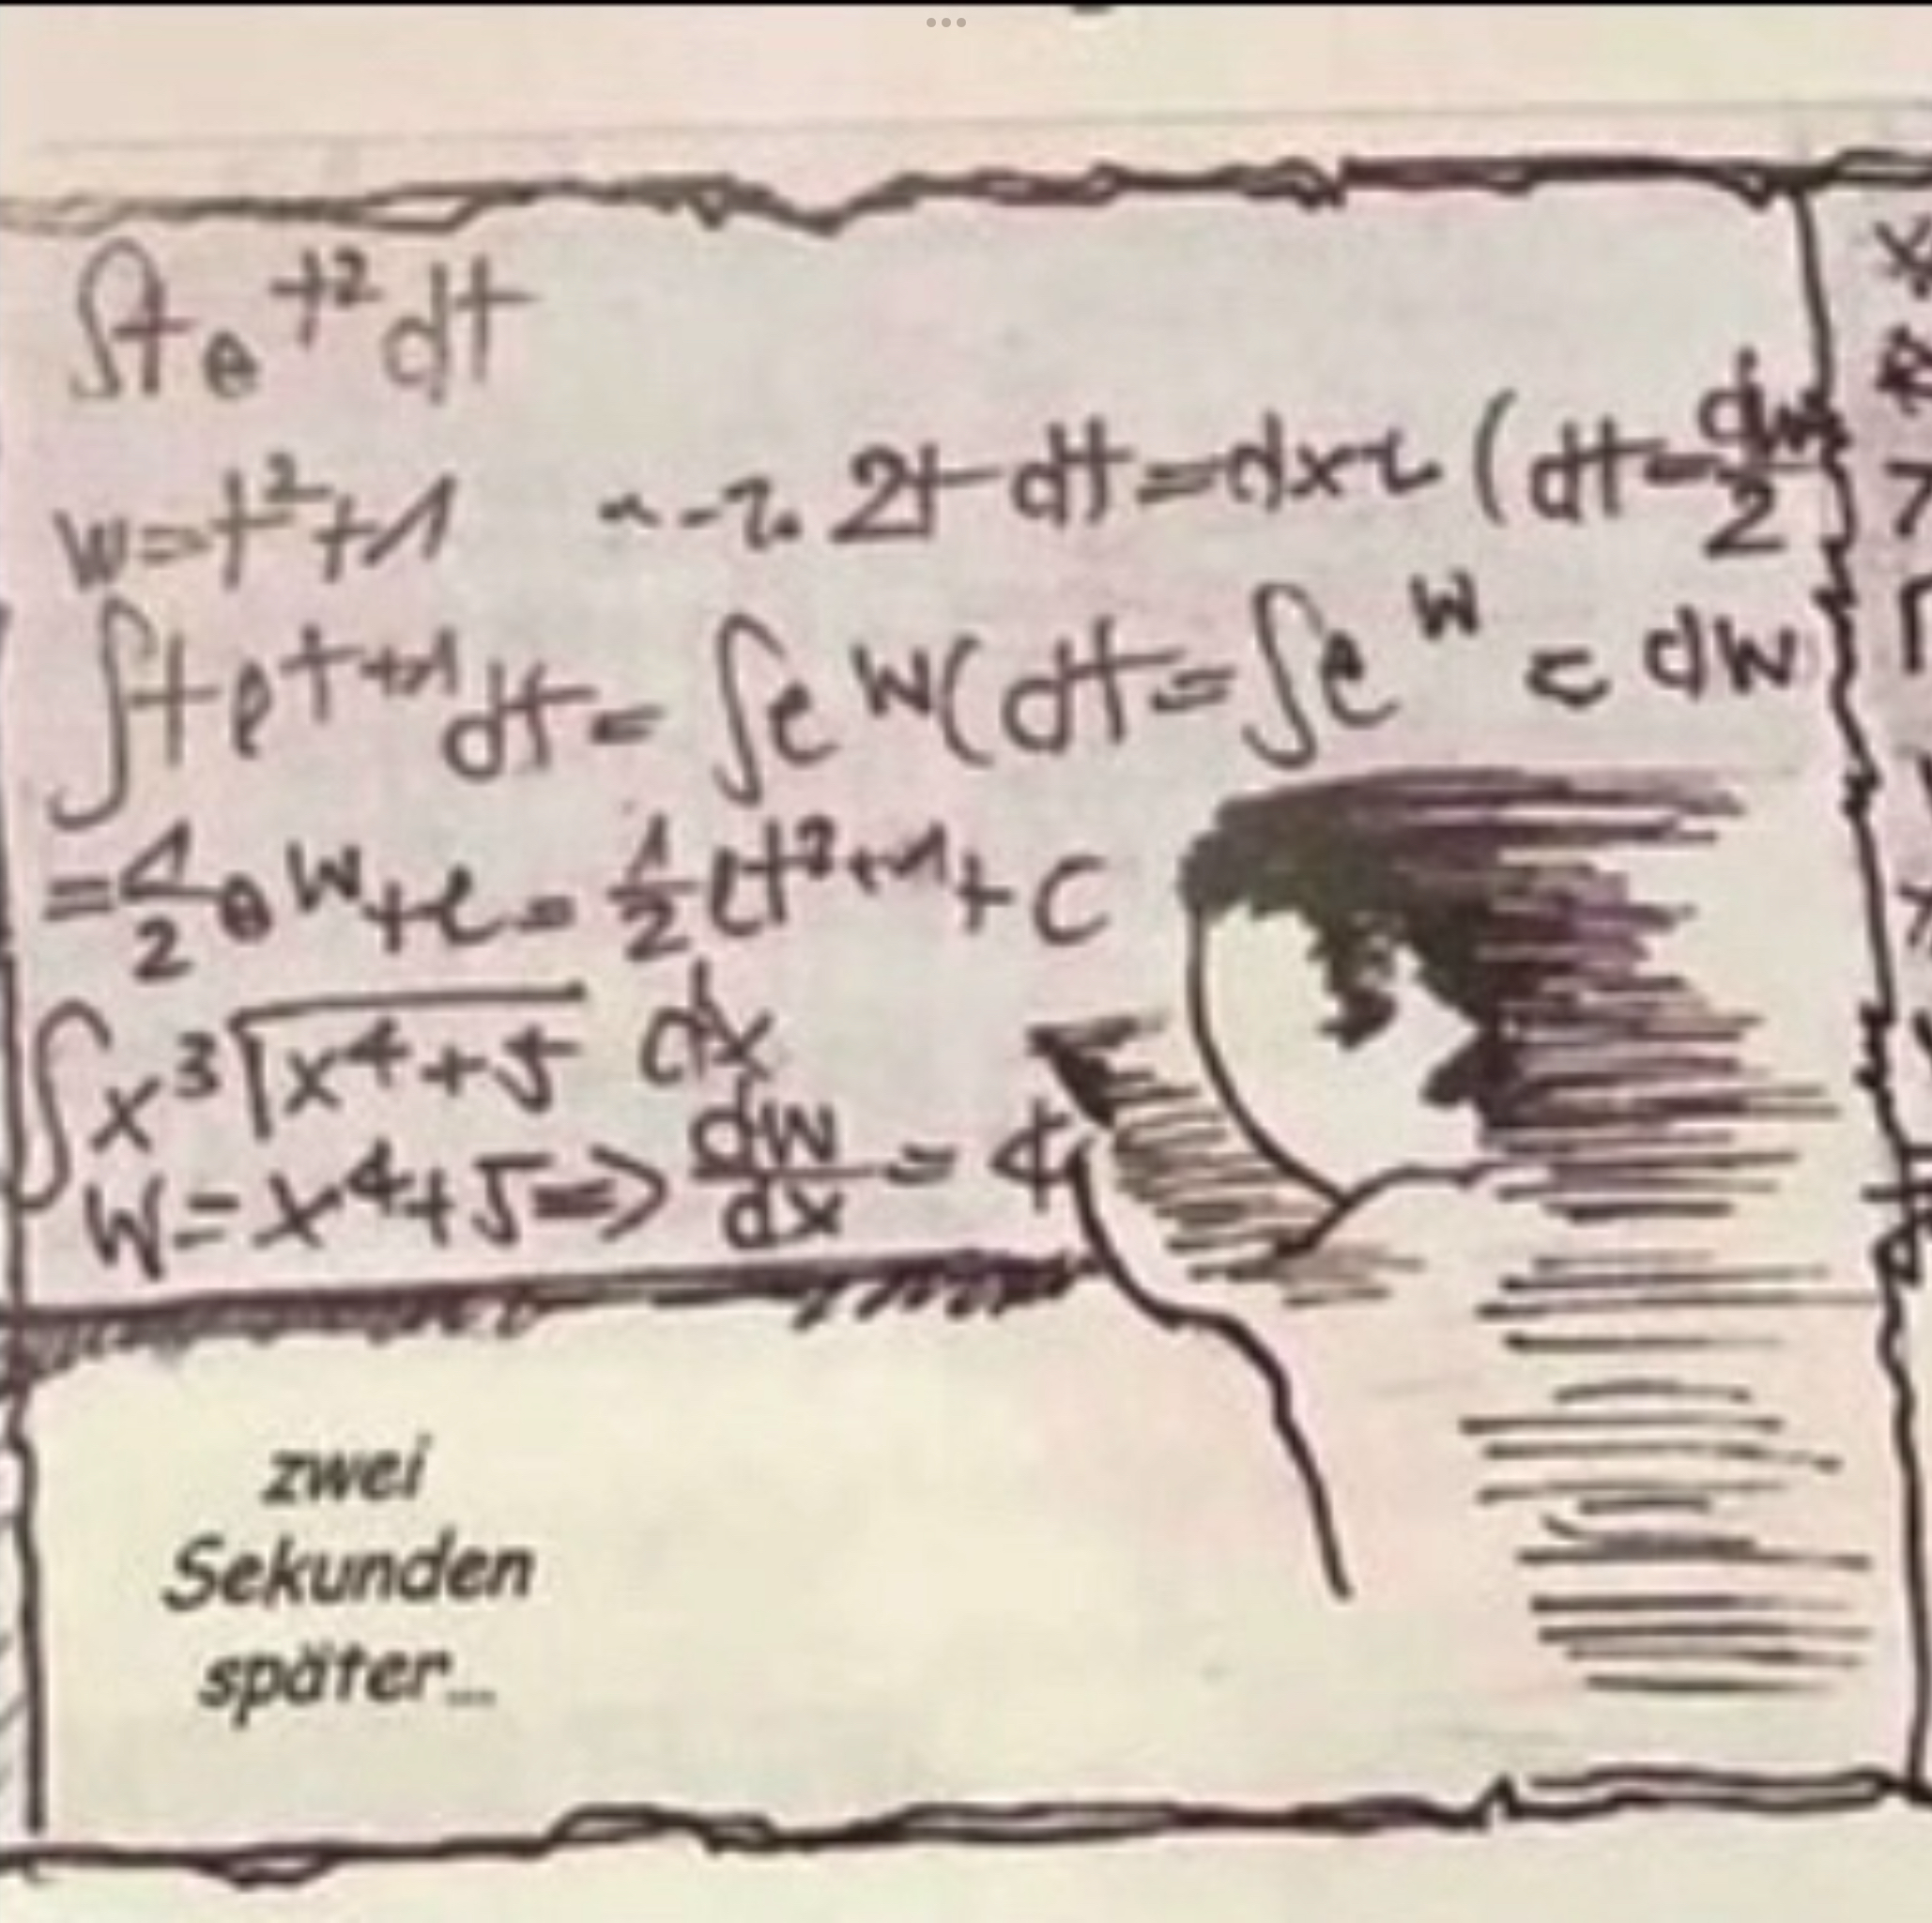
\includegraphics[width=1cm]{pictures/teacher_me_caricatur.png}}; % Adjust width and center image
\end{tikzpicture}}
}


\begin{document}
\maketitle
\tableofcontents
%\thispagestyle{empty}
\cleardoublepage
%\setcounter{page}{1}

\section{Folgen}

\subsection{Basics}
\begin{wrapfigure}{r}{0.382\textwidth}
\vspace{-2pt}
  \begin{center}
    \includegraphics[width=0.33\textwidth]{pictures/ejost}
  \end{center}
\caption{You Know my Name}
\vspace{-30pt}
\end{wrapfigure}
Das Bild \glqq You know my name (Look up the number)\grqq\ ist vom Thuner K\"unstler \textsc{Eugen Jost}.
\begin{uebenv}{eugenjost}
    Suche Gesetzm\"assigkeiten in den Zahlenfolgen und beschreibe gefundene mathematisch. Welchen Wert hat die hundertste Zahl der jeweiligen Folge? Welchen Wert hat die $k$-te Zahl der Folge?
\end{uebenv}

\begin{lsg}{eugenjost}
    \begin{enumerate}[a)]
        \item Folge der natürlichen Zahlen, $a_k=k$
        \item Folge der Kubikzahlen, $a_k=k^3$
        \item Fibonacci Folge: $a_k=a_{k-1}+a_{k-2}$ mit $a_1=1$ und $a_2=1$. Diese Folge ist häufig in der Natur zu beobachten, zum Beispiel an der Sonnenblume (ital. Girasole).
        \item Folge der Dreieckszahlen, $a_k=a_{k-1}+k$ mit $a_1=1$.
        \item Diese Folge ist ein Wortspiel. Um die nächste Zahl zu bestimmen, sagt man jeweils die Ziffern der vorhergenden Zahl auf. Beispielsweise kriegt man $a_4$ aus $a_3=21$: \glqq eine 2 und eine 1\grqq, $1211$.
        \item Das sind die vollkommenen Zahlen. Eine Zahl heisst vollkommen, wenn die Summe ihrer echten Teiler die Zahl selbst ergibt. Es ist $28=1+2+4+7+14$.
        \item Die letzte Folge ist die Telefonnummer des Künstlers.
    \end{enumerate}
\end{lsg}

\begin{uebenv}{papierfalten}
Man falte einen Bogen Papier in der Mitte und lege die beiden H\"alften aufeinander. Danach setze man dieses Prozedere mit dem gefalteten Papier fort.
\begin{enumerate}[a)]
\item Wie oft kann man das Papier h\"och\-stens falten?
\item Man denkt sich nach jeder Faltung das Papier l\"angs der Falt\-achse aufgeschnitten und die beiden H\"alf\-ten zu einem Turm aufgeschichtet. Wie hoch ist der Turm nach $2,3,4,5$ Faltungen?
<<<<<<< Updated upstream
\item Finde den Zusammenhang zwischen der Turm\-h\"ohe $h_k$ und der Anzahl Faltungen $k\in\mN$.
=======
\item Finde den Zusammenhang zwischen der Turm\-h\"ohe $h_k$ und der Anzahl Faltungen $k\in\mathbb{N}$.
>>>>>>> Stashed changes
\item Wie hoch ist der Turm nach $15,20,42$ Faltungen? Sch\"at\-ze zuerst.
\end{enumerate}
\end{uebenv}

\begin{lsg}{papierfalten}
    \begin{enumerate}[a)]
        \item Man sagt höchstens $7$ Mal, erfahrungsgemäss sind es $6$ Mal.
        \item Sei $d$ die Dicke des Papiers. Dann gilt für die Turmhöhe nach $k$ Faltungen
        $$h(k)=d\cdot 2^f.$$
        Also $h(2)=4d$, $h(3)=8d$, $h(4)=16d$, $h(5)=32d$
        \item Klassischerweise unterschätzt man die Höhe. Für $d=0.0001$ Meter ist $h(15)\approx3.28$ und $h(20)\approx104.86$ Nach $42$ Faltungen hat man, bei einer Papierdicke von $d=\unit[0.1]{mm}$, eine Höhe von $h(42)=0.0001\cdot2^{42}\approx4.398\cdot10^8$, also über $439\,800$ Kilometer. Zum Vergleich: Der Mond ist ca. $\unit[384\,444]{km}$ von der Erde entfernt. 
    \end{enumerate}
\end{lsg}

\begin{bem}
Man ahnt aus obiger Übung den Zusammenhang zwischen dieser \glqq Art\grqq\ von Folge und Exponentialfunktion. Hier ist der Unterschied zu einer Exponentialfunktion bloss, dass man nur an diskreten Werten bzw. ihren Funktionswerten interessiert ist.
\end{bem}
Eine Zahlenfolge ist eine Folge, die nur aus Zahlen besteht. Die einzelnen Zahlen der Folge nennt man \definition{Glieder}. Es ist naheliegend, jedem Glied einer bestimmten Folge seine Positionsnummer zuzuordnen.
Wir formulieren
\begin{cdef}[Folge]
Eine Folge ist eine Funktion
<<<<<<< Updated upstream
$$f:\mD\longrightarrow\mW,$$
=======
$$f:\mathbb{D}\longrightarrow\mathbb{W},$$
>>>>>>> Stashed changes
deren Definitionsmenge die Menge der nat\"urlichen Zahlen, oder eine Teilmenge davon, ist.
\end{cdef}
Besteht die Folge aus lauter reellen Zahlen, so spricht man genauer von einer Zahlenfolge.
\begin{cdef}[Zahlenfolge]
Eine Zahlenfolge ist eine Funktion
<<<<<<< Updated upstream
$$f:\D{D}\longrightarrow\D{R}$$
mit $\D{D}\subset\D{N}$.
\end{cdef}
\begin{bem}
H\"aufig wird die Bemerkung $k\in\D{N}$ weggelassen, weil sie aus dem Kontext hervorgeht. Betrachtet man Folgen, die nicht unendlich lang sind, dann sollte man die Defi\-ni\-tions\-menge explizite angeben.
\end{bem}
\begin{cdef}[Glied der Folge]
Die reellen Zahlen
$$a_1\q a_2\q a_3\q\dots\q a_{k-1}\q a_k\q a_{k+1}\q\dots$$
=======
$$f:\mathbb{D}\longrightarrow\mathbb{R}$$
mit $\mathbb{D}\subset\mathbb{N}$.
\end{cdef}
\begin{bem}
H\"aufig wird die Bemerkung $k\in\mathbb{N}$ weggelassen, weil sie aus dem Kontext hervorgeht. Betrachtet man Folgen, die nicht unendlich lang sind, dann sollte man die Defi\-ni\-tions\-menge explizite angeben.
\end{bem}
\begin{cdef}[Glied der Folge]
Die reellen Zahlen
$$a_1\quad a_2\quad a_3\quad\dots\quad a_{k-1}\quad a_k\quad a_{k+1}\quad\dots$$
>>>>>>> Stashed changes
einer Zahlenfolge heissen Glieder der Folge. $a_k$, die kurze Schreibweise von $f(k)$, heisst $k$-tes Glied der Folge.
\end{cdef}
\begin{bem}
Der Index $k$ kann also als Position in der jeweiligen Folge aufgefasst werden. $a_k$ hingegen ist der Wert, der an Position $k$ steht.
\end{bem}
<<<<<<< Updated upstream
\begin{bsps}
Zur Illustration einige Beispiele:
\begin{itemize}
\item $a_k=2k$ ist die Folge der geraden Zahlen
$$2\q4\q6\q8\q\dots,$$
denn es ist $a_1=2$, $a_2=4$, $a_3=6$, etc.
\item $a_k=2k-1$
$$1\q3\q5\q7\q\dots$$
\item $a_k=k^2$
$$1\q4\q9\q16\q\dots$$
\end{itemize}
\end{bsps}
=======
\begin{bsp}
Zur Illustration einige Beispiele:
\begin{itemize}
\item $a_k=2k$ ist die Folge der geraden Zahlen
$$2\quad4\quad6\quad8\quad\dots,$$
denn es ist $a_1=2$, $a_2=4$, $a_3=6$, etc.
\item $a_k=2k-1$
$$1\quad3\quad5\quad7\quad\dots$$
\item $a_k=k^2$
$$1\quad4\quad9\quad16\quad\dots$$
\end{itemize}
\end{bsp}
>>>>>>> Stashed changes

Die Definition einer Folge l\"asst nat\"urlich auch solche zu, die keinen Gesetzm\"assigkeiten folgen und zu denen man daher jedes Glied explizite angeben muss. Wir werden uns hier aber haupts\"achlich mit einfach zu beschreibenden Folgen befassen.

\begin{uebenv}{hunderstesglied}
Berechne die ersten vier, das hundertste und das $101$-ste Glied der Folge:

\begin{enumerate}[a)]
\item $a_k=3k-5$
\item $b_k=\frac{k}{k+1}$
\item $c_k=\left(1+\frac{1}{k}\right)^k$
\item $d_k=\sin\left(\frac{k\pi}{2}\right)$
\end{enumerate}
\end{uebenv}

\begin{lsg}{hunderstesglied}
    \begin{enumerate}[a)]
        \item $-2,1,4,7$, $295$, $300$
        \item $\frac{1}{2}, \frac{2}{3},\frac{3}{4},\frac{4}{5}$, $\frac{100}{101}$, $\frac{101}{102}$
        \item $2, \frac{9}{4}, \frac{64}{27},\frac{625}{256}$, $(\tfrac{101}{100})^{100}\approx2.7048$, $(\tfrac{102}{101})^{101}\approx2.7049$
        \item $1,0,-1,0$, $0$, $1$
    \end{enumerate}
\end{lsg}

\begin{uebenv}{mustererkennen}
Ermittle das $k$-te Glied der Folge:

\begin{enumerate}[a)]
\item $3,8,13,18,23,\dots$
\item $1,3,7,15,31,\dots$
\item $-1,4,-9,16,-25,\dots$
\item $2,6,12,20,30,\dots$
\end{enumerate}
\end{uebenv}

\begin{lsg}{mustererkennen}
    \begin{enumerate}
        \item $a_k=5k-2$
        \item $b_k=2^k-1$
        \item $c_k=(-1)^k\cdot k^2$
        \item $d_k=k(k+1)$
    \end{enumerate}
\end{lsg}

\begin{bem}
Bei vielen Zahlenfolgen ist es schwierig, die Vorschrift zu finden, mit der man das $k$-te Glied direkt berechnen kann. Jedoch kann man oft ein Bildungsgesetz erkennen, das f\"ur jede nat\"urliche Zahl $k$ die Berechnung von $a_k$ aus $a_{k-1}$ erm\"oglicht, d.h. die Berechnung des Wertes an Position $k$ anhand des Wertes der vorhergehenden Position.
\end{bem}

\subsection{Explizite und rekursive Beschreibung von Folgen}
Explizite und rekursive Definitionen von Folgen sind zwei M\"oglichkeiten, Folgen zu beschreiben.

Bei der \definition{expliziten Definition} einer Folge erh\"alt man ein beliebiges Glied sofort aus der Funktionsvorschrift, indem man direkt einsetzt. Beispielsweise ist $a_k=2k$ eine explizite Definition der Folge der geraden Zahlen.

\begin{bsp}
Eine explizite Definition von $1,3,7,15,31,\dots$
ist
$$a_k=2^k-1.$$
\end{bsp}

Bei der \definition{rekursiven Definition} einer Folge ergibt sich das $k$-te Glied aus den vorherigen Gliedern mit Hilfe einer sogenannten Rekursionsvorschrift. Bei dieser Definition m\"ussen dann auch so viele Glieder explizite vorgegeben werden, wie die Rekursionsvorschrift \glqq zum Starten\grqq\ ben\"otigt.

\begin{bsp}
Eine Rekursionsformel f\"ur $1,3,7,15,31,\dots$
ist
$$a_k=2\cdot a_{k-1}+1,\quad a_1=1.$$
\end{bsp}

\begin{bsp}
Die \textbf{Fibonacci-Folge}
<<<<<<< Updated upstream
$$1\q1\q2\q3\q5\q8\q13\q21\q\dots$$
kann durch
$$a_k=a_{k-1}+a_{k-2}\q\text{mit }a_1=1\text{ und }a_2=1$$
=======
$$1\quad1\quad2\quad3\quad5\quad8\quad13\quad21\quad\dots$$
kann durch
$$a_k=a_{k-1}+a_{k-2}\quad\text{mit }a_1=1\text{ und }a_2=1$$
>>>>>>> Stashed changes
rekursiv definiert werden.
\end{bsp}

\begin{bem}
Die Fibonacci-Folge ist \"ausserst ber\"uhmt. Benannt ist sie nach \textsc{Leonardo Fibonacci}, der damit im Jahr $1202$ das Wachstum einer Kaninchenpopulation beschrieb. Die Folge war aber schon in der Antike sowohl den Griechen als auch den Indern bekannt. Sie wird heute oft von K\"unstlern benutzt und in Film, Musik, Bildern u.\"a. verk\"orpert.
\end{bem}

\begin{bem}
F\"ur viele Zahlenfolgen k\"onnen sowohl rekursive als auch explizite Definitionen gefunden werden. Zum Beispiel ist
$$a_k=\frac{1}{\sqrt{5}}\left(\frac{1+\sqrt{5}}{2}\right)^k - \frac{1}{\sqrt{5}}\left(\frac{1-\sqrt{5}}{2}\right)^k$$
eine explizite Definition der Fibonacci-Folge, die von \textsc{de Moivre} 1718 hergeleitet wurde.
\end{bem}

\begin{uebenv}{fibonacciexplizit}
    Berechne das fünfte Glied der Fibonacci Folge mit de Moivre.
\end{uebenv}

\begin{lsg}{fibonacciexplizit}
    $\frac{1}{\sqrt{5}}\cdot((\frac{1+\sqrt{5}}{2})^5-(\frac{1-\sqrt{5}}{2})^5)=\frac{1}{\sqrt{5}}\cdot((\frac{1+5\sqrt{5}+50+50\sqrt{5}+125+25\sqrt{5}}{2})^5-(\frac{1-5\sqrt{5}+50-50\sqrt{5}+125-25\sqrt{5}}{2})^5)=\frac{1}{\sqrt{5}}\cdot(\frac{160\sqrt{5}}{32})=5$
\end{lsg}

\begin{uebenv}{bildungsgesetz}
Finde ein Bildungsgesetzt f\"ur die Folge; falls m\"oglich explizit. Beschreibe notfalls ein Bildungsverfahren.

\begin{enumerate}[a)]
\item $1,8,27,64,125,\dots$
\item $1,2,6,24,120,\dots$
\item $2,3,5,7,11,\dots$
\item $0,1,0,-1,0,1,\dots$
\end{enumerate}
\end{uebenv}

\begin{lsg}{bildungsgesetz}
    \begin{enumerate}[a)]
        \item $a_k=k^3$
        \item $b_k=k!$
        \item Folge der Primzahlen
        \item $d_k=sin(\tfrac{\pi}{2}(k-1))$
    \end{enumerate}
\end{lsg}

\begin{uebenv}{rekursivdef}
Gib eine m\"ogliche rekursive Definition f\"ur die Folge
\begin{enumerate}[a)]
\item $-7,-3,1,5,9,\dots$
\item $10,12,15,19,24,30,\dots$
\item $c_k=k\cdot2^k$
\item die Innenwinkelsumme eines $k$-Ecks $w_k$
\item die maximale Anzahl der Schnittpunkt von $k$ Geraden $s_k$
\end{enumerate}
\end{uebenv}

\begin{lsg}{rekursivdef}
    \begin{enumerate}[a)]
        \item $a_k=4k-11$
        \item $b_k=b_{k-1}+k$ mit $b_1=10$
        \item $c_k=2\cdot c_{k-1}\cdot\frac{k}{k-1}$
        \item $w_k=180^\circ\cdot(k-2)$ mit $k>2$.
        \item $s_k=\frac{k(k-1)}{2}$
    \end{enumerate}
\end{lsg}

\subsection{Die Partialsumme einer Folge}
H\"aufig ist an einer Zahlenfolge interessant, wie gross nun die Summe ihrer Glieder ist.
Hat man also eine Zahlenfolge
<<<<<<< Updated upstream
$$a_1\q a_2 \q\, a_3\q \dots$$
=======
$$a_1\quad a_2 \quad\, a_3\quad \dots$$
>>>>>>> Stashed changes
so lautet die zugeh\"orige Summe bis zum $n$-ten Glied
$$a_1+a_2+a_3+\dots+a_n.$$

Deshalb definiert man:
\begin{cdef}[Partialsumme]
Die
\marginnote{
<<<<<<< Updated upstream
\qrcode{
https://www.youtube.com/watch?v=G_PSp59zNJc}
=======
\href{https://www.youtube.com/watch?v=G_PSp59zNJc}{\qrcode{https://www.youtube.com/watch?v=G_PSp59zNJc}}
>>>>>>> Stashed changes
}
$k$-te Partialsumme der ersten $k$ oder aller Glieder einer Zahlenfolge ist die Summe
$$s_n=a_1+a_2+\ldots+a_{k-1}+a_n=:\sum_{k=1}^na_k$$
\end{cdef}

\begin{uebenv}{gausstrick}
Berechne die erste, dritte, 100., $n$-te Partialsumme der Folge
<<<<<<< Updated upstream
$$1\q2\q3\q4\q\dots$$
=======
$$1\quad2\quad3\quad4\quad\dots$$
>>>>>>> Stashed changes
Tipp: Verwende Kombinatorik oder den Trick von C.F.~Gauss.
\end{uebenv}

\begin{lsg}{gausstrick}
    $s_1=1$ und $s_3=6$. Für $1+2+\dots+100$ addiert man paarweise Summanden so, dass deren Paketgrösse gleich ist: $(1+100), (2+99), (3+98),\dots$. Von diesen Paketen hat man $50$ Stück. Also ist $1+2+\dots+100=101\cdot50=5050$. Analog findet man $s_n=(1+n)\cdot\frac{n}{2}$.
\end{lsg}

\begin{bem}
Wie oben erwähnt, schreibt man eine Summe auch wie folgt:
$$a_1+a_2+a_3+\dots+a_n = \sum_{k=1}^{n}a_k.$$
Dabei schreibt man also ein grosses $\Sigma$ (Sigma), um anzudeuten, dass es sich um eine Summe handelt. Unterhalb dieses Sigmas wird notiert, bei welchem nat\"urlichen Wert die laufende Variable (hier $k$) startet. Dieses $k$ wird solange um $1$ erh\"oht, bis es die obere Grenze $n$ erreicht hat. Zwischen den Erh\"ohungen wird immer ein $+$-Zeichen gesetzt.
\end{bem}

<<<<<<< Updated upstream
\begin{bsps}
=======
\begin{bsp}
>>>>>>> Stashed changes
\begin{align}
\notag
\sum_{k=1}^{n}k &=1+2+3+4+\dots +n\\ \notag
\sum_{k=1}^{n}k^2 &=1^2+2^2+3^2+4^2+\dots+n^2\\ \notag
\sum_{k=100}^{999}k &=100+101+102+\dots+999
\end{align}
<<<<<<< Updated upstream
\end{bsps}

\begin{bem}
Man kann aus einer Zahlenfolge eine neue zusammenstellen, welche einfach aus den verschiedenen Teilsummen der urspr\"unglichen Zahlenfolge besteht. Wenn man beispielsweise die Zahlenfolge
$$1\q2\q3\q4\q5\dots$$
anschaut, dann ist ihre erste Teilsumme $s_1=1$, ihre zweite $s_2=3$, die dritte $s_3=6$, die vierte $s_4=10$, etc. Man kann also eine Folge der Teilsummen
$$1\q3\q6\q10\q15\q21\dots$$
=======
\end{bsp}

\begin{bem}
Man kann aus einer Zahlenfolge eine neue zusammenstellen, welche einfach aus den verschiedenen Teilsummen der urspr\"unglichen Zahlenfolge besteht. Wenn man beispielsweise die Zahlenfolge
$$1\quad2\quad3\quad4\quad5\dots$$
anschaut, dann ist ihre erste Teilsumme $s_1=1$, ihre zweite $s_2=3$, die dritte $s_3=6$, die vierte $s_4=10$, etc. Man kann also eine Folge der Teilsummen
$$1\quad3\quad6\quad10\quad15\quad21\dots$$
>>>>>>> Stashed changes
bestehend aus den einzelnen Teilsummen
$$s_k=\sum_{i=1}^{k}i$$
bilden.
\end{bem}

\begin{uebenv}{erstepartialsummen}
Stelle folgenden Ausdruck mit einem einzigen Term dar
$$s_k=\frac{1}{1\cdot2}+\frac{1}{2\cdot3}+\frac{1}{3\cdot4}+\frac{1}{4\cdot5}+\dots+\frac{1}{k\cdot(k+1)}$$
Berechne dazu erst einmal die Summe der ersten paar Glieder, also $s_1, s_2, s_3,\dots$, explizite, und versuche dann eine Formel f\"ur obigen Ausdruck zu erraten, die den Wert von $s_k$ explizite angibt. Versuche abzuschätzen, gegen welchen Wert diese Summe strebt, wenn $k$ sehr gross wird.
\end{uebenv}

\begin{lsg}{erstepartialsummen}
    $s_1=\frac{1}{2}$, $s_2=\frac{2}{3}$, $s_3=\frac{3}{4}$, vermutlich $s_k=\frac{k}{k+1}$. Für $k\to\infty$ ist $\frac{k}{k+1}\to\frac{k}{k}=1$
\end{lsg}

\begin{uebenv}{summezweierpotenzen}
Wie vorhergehende Übung, aber mit dem Ausdruck
$$s_k=1+\frac{1}{2}+\frac{1}{4}+\frac{1}{8}+\dots+a_k$$
Finde zuerst eine Darstellung f\"ur $a_k$. Gegen welchen Wert strebt die Summe für $k\to\infty$
\end{uebenv}

\begin{lsg}{summezweierpotenzen}
    $a_k=\frac{1}{2^{k-1}}$. $s_1=1$, $s_2=\frac{3}{2}$, $s_3=\frac{7}{4}$, $s_4=\frac{15}{8}$ und vermutlich $s_k=\frac{2^k-1}{2^{k-1}}$. Für $k\to\infty$ ist $\frac{2^k-1}{2^{k-1}}\to\frac{2^k}{2^{k-1}}=2$
\end{lsg}

Im Folgenden werden wir uns fast ausschliesslich auf zwei Typen von Zahlenfolgen beschr\"anken. N\"amlich einerseits auf Folgen, bei denen der \glqq Abstand\grqq\ zweier aufeinander folgender Glieder konstant ist (verwandt mit affinen Funktionen), und andererseits auf Folgen, bei denen der Quotient zweier aufeinander folgender Glieder konstant ist (verwandt mit Exponentialfuntionen).

\clearpage

\section{Arithmetische Folgen \&\ Reihen}

\begin{cdef}[Arithmetische Folge]
Eine
\marginnote{
<<<<<<< Updated upstream
\qrcode{
https://www.youtube.com/watch?v=zGVcjrRe1Hg}
}
arithmetische Folge ist eine Zahlenfolge, deren Glieder der Rekursionsformel
$$a_{k+1}=a_k+d\q (k\in\mN, d=\text{konstant})$$
=======
\href{https://www.youtube.com/watch?v=zGVcjrRe1Hg}{\qrcode{https://www.youtube.com/watch?v=zGVcjrRe1Hg}}
}
arithmetische Folge ist eine Zahlenfolge, deren Glieder der Rekursionsformel
$$a_{k+1}=a_k+d\quad (k\in\mathbb{N}, d=\text{konstant})$$
>>>>>>> Stashed changes
gen\"ugen.
\end{cdef}

\begin{bem}
Der Name arithmetische Folge ist dadurch motiviert, dass jedes Glied --- ausser das erste und gegebenenfalls das letzte --- gleich dem arithmetischen Mittel der Nachbarglieder ist.
\end{bem}

\begin{uebenv}{namearithmetisch}
Zeige die G\"ultigkeit der obigen Bemerkung.
\end{uebenv}

\begin{lsg}{namearithmetisch}
    Es ist $\frac{a_{k-1}+a_{k+1}}{2}=\frac{a_k-d+a_k+d}{2}=\frac{2a_k}{2}=a_k$
\end{lsg}

\begin{bsp}
Die Folge der ungeraden nat\"urlichen Zahlen ist arithmetisch mit $d=2$.
<<<<<<< Updated upstream
$$1\q3\q5\q7\q9\q\dots$$
=======
$$1\quad3\quad5\quad7\quad9\quad\dots$$
>>>>>>> Stashed changes
\end{bsp}

\begin{csatz}
F\"ur eine arithmetische Folge gelten
\begin{align}
a_k&=a_1+(k-1)\cdot d\label{arithglied}\\
s_k&=k\cdot\frac{a_1+a_k}{2}\label{arithsum}
\end{align}
\end{csatz}

\begin{proof}[Beweis]
(\ref{arithglied}) ist eine \glqq Pf\"ostchen-Überlegung\grqq. F\"ur (\ref{arithsum}) nimmt man den Trick von Gauss.
\end{proof}

\begin{uebenv}{dreierzahlen}
Berechne die Summe aller Dreierzahlen von $81$ bis $1020$.
\end{uebenv}

\begin{lsg}{dreierzahlen}
    Es ist $a_1=81$ und $a_n=1020$. Somit folgt $1020=81+(k-1)\cdot3\Leftrightarrow 3k=942\Leftrightarrow k=314$. Also schliessen wir $s_{314}=(81+1020)\cdot157=16\,515$
\end{lsg}

\begin{uebenv}{freierfall}
Ein frei fallender K\"orper legt in der ersten Sekunde $\unit[5]{m}$ und in jeder folgenden Sekunde $\unit[10]{m}$ mehr als in der jeweils vorangegangenen Sekunde zur\"uck.
\begin{enumerate}[a)]
\item Welche Strecke legt er in der 13-ten Sekunde zur\"uck?
\item Welche Strecke f\"allt er in $\unit[13]{Sekunden}$?
\item Wie viele Sekunden braucht er f\"ur $\unit[1805]{m}$?
\end{enumerate}
\end{uebenv}

\begin{lsg}{freierfall}
    \begin{enumerate}[a)]
        \item $a_1=5$, $a_2=15$, $a_3=25$, \dots, $a_{13}=5+12\cdot10=125$ Meter.
        \item $s_{13}=(5+125)\cdot\frac{13}{2}=845$ Meter
        \item $1805=(5+a_n)\cdot\frac{n}{2}=(5+5+(n-1)\cdot10)\cdot\frac{n}{2}=10n\cdot\frac{n}{2}=5n^2$. Also $n^2=361$ und damit $n=19$ Sekunden. Die negative Lösung ist sinnlos.
    \end{enumerate}
\end{lsg}

\section{Geometrische Folgen \&\ Reihen}

\begin{cdef}[geometrische Folge]
Eine
\marginnote{
<<<<<<< Updated upstream
\qrcode{
https://www.youtube.com/watch?v=b0rjVBStXGo}
}
geometrische Folge ist eine Zahlenfolge, deren Glieder der Rekursionsformel
$$a_{k+1}=a_k\cdot q\q(k\in\mN, q=\text{konstant})$$
=======
\href{https://www.youtube.com/watch?v=b0rjVBStXGo}{\qrcode{https://www.youtube.com/watch?v=b0rjVBStXGo}}
}
geometrische Folge ist eine Zahlenfolge, deren Glieder der Rekursionsformel
$$a_{k+1}=a_k\cdot q\quad(k\in\mathbb{N}, q=\text{konstant})$$
>>>>>>> Stashed changes
gen\"ugen.
\end{cdef}

\begin{bem}
Der Name geometrische Folge ist dadurch motiviert, dass jedes Glied --- ausser das erste und gegebenenfalls das letzte --- betragsmässig gleich dem geometrischen Mittel der Nachbarglieder ist.
\end{bem}

\begin{uebenv}{namegeometrisch}
Zeige die G\"ultigkeit der obigen Bemerkung.
\end{uebenv}

\begin{lsg}{namegeometrisch}
    $\sqrt{a_{k-1}\cdot a_{k+1}}=\sqrt{\frac{a_k}{q}\cdot a_kq}=\sqrt{a_k^2}=|a_k|$
\end{lsg}

\begin{bsp}
Die Folge der Zweierpotenzen mit nat\"urlichen Exponenten ist geometrisch mit $q=2$.
<<<<<<< Updated upstream
$$2\q4\q8\q16\q32\q\dots$$
=======
$$2\quad4\quad8\quad16\quad32\quad\dots$$
>>>>>>> Stashed changes
\end{bsp}

\begin{csatz}[GF Formeln]
F\"ur eine geometrische Folge gelten
\begin{align}
a_k&=a_1\cdot q^{k-1}\label{geomglied}\\
s_k&=a_1\cdot\frac{q^k-1}{q-1}\label{geomsum}
\end{align}
\end{csatz}

\begin{proof}[Beweis]
(\ref{geomglied}) ist wiederum eine \glqq Pf\"ostchen-\"Uberlegung\grqq. Wir zeigen (\ref{geomsum}) und nehmen dazu an, dass die Folge endlich sei.
\begin{align*}
s_k&=a_1+a_2+a_3+\ldots+a_k\\
&=a_1+a_1\cdot q+a_1\cdot q^2+\ldots+a_1\cdot q^{k-1}
\end{align*}
Multipliziert man diese Gleichung mit $q$ folgt
$$s_k\cdot q=a_1\cdot q+a_1\cdot q^2+a_1\cdot q^3+\ldots+a_1\cdot q^k$$
Nun subtrahieren wir $s_k$ von $s_k\cdot q$ und erhalten
$$s_k\cdot q-s_k=s_k(q-1)=a_1\cdot q^k-a_1=a_1(q^k-1)$$
Daraus folgt unmittelbar
$$s_k=\frac{a_1(q^k-1)}{q-1}$$
und damit die Behauptung.
\end{proof}

\begin{uebenv}{alternierendezweierpotenzen}
Berechne
$$-2+4-8+16-\dots+4096.$$
\end{uebenv}

\begin{lsg}{alternierendezweierpotenzen}
    $q=-2$ klar. $4096=(-2)\cdot(-2)^{k-1}=(-2)^k\Leftrightarrow k=\log_2(4096)=12$. Es folgt $s_{12}=(-2)\cdot\frac{(-2)^{12}-1}{(-2)-1}=2730$
\end{lsg}

\begin{uebenv}{folgezweischeneinsundzwei}
Eine geometrische Folge besteht aus 10 positiven Gliedern, beginnt mit $1$ und endet mit $2$. Bestimme das Bildungsgesetz dieser Folge und berechne die zugeh\"orige Partialsumme aller Glieder.
\end{uebenv}

\begin{lsg}{folgezwischeneinsundzwei}
    $a_1=1$ und $a_{10}=2$. Damit $2=1\cdot q^9\Leftrightarrow q=\sqrt[9]{2}$, also $a_k=(\sqrt[9]{2})^{k-1}=2^\frac{k-1}{9}$. Die Partialsumme ist $s_{10}=1\cdot\frac{(\sqrt[9]{2})^{10}-1}{\sqrt[9]{2}-1}\approx14.5$
\end{lsg}

\clearpage

\section{\"Ubungen zu arithmetischen und geometrischen Folgen}

\begin{uebenv}{rohreschichten}
Es sind 60 Rohre so zu stapeln, dass jede Schicht auf L\"ucke mit der darunter liegenden Schicht liegt; die oberste Schicht soll aus vier Rohren bestehen. Wie viele Rohre m\"ussen in die unterste Schicht gelegt werden, und wie viele Schichten hat der Stapel? Wie hoch ist er, wenn die Rohre einen Durchmesser von $\unit[20]{cm}$ haben?
\end{uebenv}

\begin{lsg}{rohreschichten}
Ich stelle mir schematisch die Rohre wie folgt aufeinandergestapelt vor.

\begin{center}
\begin{tikzpicture}
% Define the radius of the circles
\def\radius{0.5}

% Draw the circles in each row
\foreach \row/\num in {0/0, 1/1, 2/2, 3/3, 4/4} {
    \foreach \col in {0,...,\num} {
        \draw (\col - \num/2 + 0.5, -\row * \radius * 1.85) circle (\radius);
    }
}

% Connect the outer circles to form an equilateral triangle
\draw (-1.55, -3.7) -- (2.55, -3.7) -- (0.5, 0.05) -- cycle;
\end{tikzpicture}
\end{center}

Jetzt bestehe die oberste Schicht aus $a_1=4$ Rohren und $d=1$. Wir wissen $s_n=60=(4+a_n)\cdot\frac{n}{2}=(4+(4+(n-1))\cdot\frac{n}{2}=\frac{n^2}{2}+\frac{7}{2}n$. Es folgt $0=n^2+7n-120=(n+15)(n-8)$ und damit $n=8$ Schichten. In der untersten Reihe sind dann $a_8=4+7\cdot1=11$ Rohre.

Für die Höhe rechnen wir die Höhe des grossen gleichseitigen Dreiecks minus die Höhe des kleinen imaginären Spitzedreieck plus einmal den Radius oben und unten: $10\cdot20\cdot\frac{\sqrt{3}}{2}-3\cdot20\cdot\frac{\sqrt{3}}{2}+20$ und erhalten $20+70\sqrt{3}\approx1.41$ Meter.
\end{lsg}

\begin{uebenv}{kalium}
F\"ur manche medizinische Diagnosen wird das radioaktive Kalium\-isotop $^{42}$K benutzt. Es verliert pro Stunde $5.42\%$ seiner Intensit\"at. Welchen Prozentsatz verliert es nach drei Stunden?
\end{uebenv}

\begin{lsg}{kalium}
    Nach drei Stunden hat es $1-0.9458^3\approx15.4\%$ verloren.
\end{lsg}

\begin{uebenv}{afundgf}
$a, b, c$ bilden in dieser Reihenfolge eine arithmetische Folge mit der Summe $3$; in der Reihenfolge $b, c, a$ bilden sie eine geometrische Folge. Berechne die drei Zahlen, wenn $a\neq b\neq c$.
\end{uebenv}

\begin{lsg}{afundgf}
    Wir haben $a+b+c=3=3b\Leftrightarrow b=1$ und $b+bq+bq^2=3\Leftrightarrow q^2+q-2=0\Leftrightarrow q_1=-2,q_2=1$. Also $a,b,c=4,1,-2$ oder $1,1,1$.
\end{lsg}

\begin{uebenv}{reiskoerner}
In
\marginnote{
<<<<<<< Updated upstream
\qrcode{
https://www.youtube.com/watch?v=UGOdwBEIbWc}
}
einer Erz\"ahlung des Persers \textsc{Ibn Khallikan} aus dem 13.Jahrhundert lesen wir: \glqq In jener Zeit, als der indische Herrscher \textsc{Shihram} seine Untertanen unm\"assig tyrannisierte, erfand der Weise \textsc{Sissa Ibn Dahir} zur Belehrung des K\"onigs das Schachspiel, um ihm nachzuweisen, wie wichtig f\"ur einen Herrscher seine Untertanen sind. Als Dank f\"ur die Erleuchtung bot der K\"onig \textsc{Sissa} seine Sch\"atze an und stellte ihm einen Wunsch frei. Der Weise w\"unschte sich soviel Weizen, wie sich auf dem Schachbrett folgendermassen angeordnet ergibt: Auf das erste Feld des Schachbrettes 1 Reiskorn, auf das zweite Feld 2 Reisk\"orner, auf das dritte Feld 4 K\"orner etc., auf jedem Feld doppelt so viele wie auf dem vorhergehenden.\grqq
\begin{enumeratea}
\item Wie viele Reisk\"orner sind dies insgesamt?
\item Wie lange w\"are ein Zug, der diese Reismenge transportieren m\"usste, wenn ein G\"uterwagen von $\unit[10]{m}$ L\"ange $\unit[10]{Tonnen}$ Reis laden kann und  $18$ K\"orner $\unit[1]{g}$ ergeben?
\item Welche H\"ohe h\"atte ein Reisteppich, wenn man die Schweiz damit bedecken w\"urde? (Nimm z.B. ein zylindrisches Reiskorn mit Durchmesser $\unit[2]{mm}$ und H\"ohe $\unit[1]{cm}$.)
\end{enumeratea}
=======
\href{https://www.youtube.com/watch?v=UGOdwBEIbWc}{\qrcode{https://www.youtube.com/watch?v=UGOdwBEIbWc}}
}
einer Erz\"ahlung des Persers \textsc{Ibn Khallikan} aus dem 13.Jahrhundert lesen wir: \glqq In jener Zeit, als der indische Herrscher \textsc{Shihram} seine Untertanen unm\"assig tyrannisierte, erfand der Weise \textsc{Sissa Ibn Dahir} zur Belehrung des K\"onigs das Schachspiel, um ihm nachzuweisen, wie wichtig f\"ur einen Herrscher seine Untertanen sind. Als Dank f\"ur die Erleuchtung bot der K\"onig \textsc{Sissa} seine Sch\"atze an und stellte ihm einen Wunsch frei. Der Weise w\"unschte sich soviel Weizen, wie sich auf dem Schachbrett folgendermassen angeordnet ergibt: Auf das erste Feld des Schachbrettes 1 Reiskorn, auf das zweite Feld 2 Reisk\"orner, auf das dritte Feld 4 K\"orner etc., auf jedem Feld doppelt so viele wie auf dem vorhergehenden.\grqq
\begin{enumerate}[a)]
\item Wie viele Reisk\"orner sind dies insgesamt?
\item Wie lange w\"are ein Zug, der diese Reismenge transportieren m\"usste, wenn ein G\"uterwagen von $\unit[10]{m}$ L\"ange $\unit[10]{Tonnen}$ Reis laden kann und  $18$ K\"orner $\unit[1]{g}$ ergeben?
\item Welche H\"ohe h\"atte ein Reisteppich, wenn man die Schweiz damit bedecken w\"urde? (Nimm z.B. ein zylindrisches Reiskorn mit Durchmesser $\unit[2]{mm}$ und H\"ohe $\unit[1]{cm}$.)
\end{enumerate}
>>>>>>> Stashed changes
\end{uebenv}

\begin{lsg}{reiskoerner}
    \begin{enumerate}[a)]
        \item Wir berechnen $1+2+4+8+\dots+2^{63}=1\cdot\frac{2^{64}-1}{2-1}=2^{64}-1=18\,446\,744\,073\,709\,551\,615$ Reiskörner.
        \item Ich rechne mit einem Reiskorn mehr. Wir bekommen $\frac{2^{64}}{18\cdot10^7}$ 10t-Einheiten, also abgerundet ca. $10^{11}$ Wagons, die aneinander gereiht dann $10^{9}$ Kilometer lang wären. Als Vergleich erinnern wir uns an den Abstand Erde-Sonne, der etwas weniger als $1.5\cdot10^8$ Kilometer beträgt.
        \item Das Volumen ist $2^{64}\cdot0.01\cdot0.001^2\pi$ Kubikmeter. Das teilen wir durch die Fläche der Schweiz $41\,291\cdot1000^2$ in Quadratmeter und kriegen die Höhe $14.5$ Meter.
    \end{enumerate}
\end{lsg}

\begin{uebenv}{quadrate}
Die Figuren sind aus Quadraten zusammengesetzt wie in Abbildung \ref{ueb:quadrate} auf Seite \pageref{ueb:quadrate}.
\begin{figure}
\centering
\definecolor{zzttqq}{rgb}{0.6,0.2,0}
\definecolor{cqcqcq}{rgb}{0.75,0.75,0.75}
\scalebox{1.2}{
\begin{tikzpicture}[line cap=round,line join=round,x=0.45cm,y=0.45cm]
\draw [color=cqcqcq,dash pattern=on 2pt off 2pt, xstep=0.45cm,ystep=0.45cm] (-2.6,-1.28) grid (11.6,6.3);
\clip(-2.6,-1.28) rectangle (11.6,6.3);
\fill[line width=1.6pt,color=zzttqq,fill=zzttqq,fill opacity=0.15] (-2,2) -- (-1,2) -- (-1,3) -- (-2,3) -- cycle;
\fill[line width=1.6pt,color=zzttqq,fill=zzttqq,fill opacity=0.15] (2,3) -- (2,4) -- (3,4) -- (3,3) -- (4,3) -- (4,2) -- (3,2) -- (3,1) -- (2,1) -- (2,2) -- (1,2) -- (1,3) -- cycle;
\fill[line width=1.6pt,color=zzttqq,fill=zzttqq,fill opacity=0.15] (6,3) -- (7,3) -- (7,4) -- (8,4) -- (8,5) -- (9,5) -- (9,4) -- (10,4) -- (10,3) -- (11,3) -- (11,2) -- (10,2) -- (10,1) -- (9,1) -- (9,0) -- (8,0) -- (8,1) -- (7,1) -- (7,2) -- (6,2) -- cycle;
\draw [line width=1.6pt,color=zzttqq] (-2,2)-- (-1,2);
\draw [line width=1.6pt,color=zzttqq] (-1,2)-- (-1,3);
\draw [line width=1.6pt,color=zzttqq] (-1,3)-- (-2,3);
\draw [line width=1.6pt,color=zzttqq] (-2,3)-- (-2,2);
\draw [line width=1.6pt,color=zzttqq] (2,3)-- (2,4);
\draw [line width=1.6pt,color=zzttqq] (2,4)-- (3,4);
\draw [line width=1.6pt,color=zzttqq] (3,4)-- (3,3);
\draw [line width=1.6pt,color=zzttqq] (3,3)-- (4,3);
\draw [line width=1.6pt,color=zzttqq] (4,3)-- (4,2);
\draw [line width=1.6pt,color=zzttqq] (4,2)-- (3,2);
\draw [line width=1.6pt,color=zzttqq] (3,2)-- (3,1);
\draw [line width=1.6pt,color=zzttqq] (3,1)-- (2,1);
\draw [line width=1.6pt,color=zzttqq] (2,1)-- (2,2);
\draw [line width=1.6pt,color=zzttqq] (2,2)-- (1,2);
\draw [line width=1.6pt,color=zzttqq] (1,2)-- (1,3);
\draw [line width=1.6pt,color=zzttqq] (1,3)-- (2,3);
\draw [line width=1.6pt,color=zzttqq] (6,3)-- (7,3);
\draw [line width=1.6pt,color=zzttqq] (7,3)-- (7,4);
\draw [line width=1.6pt,color=zzttqq] (7,4)-- (8,4);
\draw [line width=1.6pt,color=zzttqq] (8,4)-- (8,5);
\draw [line width=1.6pt,color=zzttqq] (8,5)-- (9,5);
\draw [line width=1.6pt,color=zzttqq] (9,5)-- (9,4);
\draw [line width=1.6pt,color=zzttqq] (9,4)-- (10,4);
\draw [line width=1.6pt,color=zzttqq] (10,4)-- (10,3);
\draw [line width=1.6pt,color=zzttqq] (10,3)-- (11,3);
\draw [line width=1.6pt,color=zzttqq] (11,3)-- (11,2);
\draw [line width=1.6pt,color=zzttqq] (11,2)-- (10,2);
\draw [line width=1.6pt,color=zzttqq] (10,2)-- (10,1);
\draw [line width=1.6pt,color=zzttqq] (10,1)-- (9,1);
\draw [line width=1.6pt,color=zzttqq] (9,1)-- (9,0);
\draw [line width=1.6pt,color=zzttqq] (9,0)-- (8,0);
\draw [line width=1.6pt,color=zzttqq] (8,0)-- (8,1);
\draw [line width=1.6pt,color=zzttqq] (8,1)-- (7,1);
\draw [line width=1.6pt,color=zzttqq] (7,1)-- (7,2);
\draw [line width=1.6pt,color=zzttqq] (7,2)-- (6,2);
\draw [line width=1.6pt,color=zzttqq] (6,2)-- (6,3);
\end{tikzpicture}
}
\caption{Quadrate}\label{ueb:quadrate}
\end{figure}
Stelle eine Formel auf f\"ur die Anzahl $a(k)$ der Quadrate, die in der $k$-ten Figur vorhanden sind.
\end{uebenv}

\begin{lsg}{quadrate}
    Die Folge ist $1,5,13,\dots$. Man hat für das $k$-te Gebilde $a_k=2k-1+2\cdot(k-1)^2=2k^2-2k+1$.
\end{lsg}

\begin{uebenv}{maturafolgen}
In
\marginnote{
<<<<<<< Updated upstream
\qrcode{
https://www.youtube.com/watch?v=AJtWxcZNq28}
=======
\href{https://www.youtube.com/watch?v=AJtWxcZNq28}{\qrcode{https://www.youtube.com/watch?v=AJtWxcZNq28}}
>>>>>>> Stashed changes
}
der Randnotiz findet man ein Video zur Matura Mathematik Aufgabe Folgen und Reihen von 2013. Darin seht ihr die Aufgabe und eine mögliche Lösung kommentiert.
\end{uebenv}

\begin{lsg}{maturafolgen}
    \href{https://www.youtube.com/watch?v=AJtWxcZNq28}{Youtube Video mit Kommentar zur Aufgabe}
\end{lsg}

\clearpage

\section{Grenzwerte}
\subsection{Konvergenz und bestimmte Divergenz}
\begin{wrapfigure}{r}{0.382\textwidth}
\vspace{-23pt}
  \begin{center}
    \includegraphics[width=0.36\textwidth]{pictures/limit}
  \end{center}
\vspace{-20pt}
\end{wrapfigure}
Bisher haben wir nur die Anfangsglieder einer Folge betrachtet. Wir wenden uns in diesem Kapitel den Gliedern mit hohen Nummern zu und werden versuchen, Aussagen \"uber ihr Verhalten zu machen, wenn $n$ gegen Unendlich strebt (schreibe: $n\to\infty$).
<<<<<<< Updated upstream
Wir schreiben f\"ur eine Zahlenfolge $f:\mN\to\mR, k\mapsto f(k)$ kurz $<a_k>$.
=======
Wir schreiben f\"ur eine Zahlenfolge $f:\mathbb{N}\to\mathbb{R}, k\mapsto f(k)$ kurz $<a_k>$.
>>>>>>> Stashed changes

\begin{uebenv}{nahanslimit}
Berechne f\"ur $k=10,11,10^3,10^3+1,10^6,10^6+1$ die Glieder der Zahlenfolge mit

\begin{enumerate}[a)]
\item $a_k=5+\frac{1}{k}$
\item $b_k=(-1)^k\cdot\frac{3000}{k}$
\item $c_k=k^3$
\item $d_k=1+(-1)^k$
\end{enumerate}
\end{uebenv}

\begin{lsg}{nahanslimit}
    \begin{enumerate}[a)]
        \item $a_{10}=\frac{51}{10}$, $a_{11}=\frac{28}{5}$,$a_{1000}=\frac{5001}{1000}$, $a_{1001}=\frac{5006}{1001}$, $a_{10^6}=\frac{5\,000\,001}{10^6}$, $a_{10^6+1}=\frac{5\,000\,006}{10^6+1}$
        \item $b_{10}=300$, $b_{11}=-\frac{3000}{11}$,$b_{1000}=3$, $b_{1001}=-\frac{3000}{1001}$, $b_{10^6}=\frac{3}{1000}$, $b_{10^6+1}=-\frac{3000}{10^6+1}$
        \item $c_{10}=10^3$, $c_{11}=11^3$,$c_{1000}=10^9$, $b_{1001}=-1001^3$, $b_{10^6}=10^{18}$, $b_{10^6+1}=(10^6+1)^3$
        \item $d_{10}=2$, $d_{11}=0$,$d_{1000}=2$, $d_{1001}=0$, $d_{10^6}=2$, $d_{10^6+1}=0$
    \end{enumerate}
\end{lsg}

<<<<<<< Updated upstream
Wir k\"onnen also das Verhalten von Folgen f\"ur grosse $k\in\mN$ in drei wesentliche F\"alle aufteilen.
=======
Wir k\"onnen also das Verhalten von Folgen f\"ur grosse $k\in\mathbb{N}$ in drei wesentliche F\"alle aufteilen.
>>>>>>> Stashed changes
\begin{itemize}
\item[A] Die Glieder der Folge streben f\"ur $k\to\infty$ genau einer reellen Zahl, einem Grenzwert, zu.
\item[B] Die Glieder der Folge werden f\"ur $k\to\infty$ betragsm\"assig gr\"osser als jede noch so grosse Zahl.
\item[C] Die Glieder der Folge verhalten sich nicht so wie in den beiden andern F\"allen.
\end{itemize}
Im Fall A nennt man die Folge \definition{konvergent}, im Fall B bestimmt \definition{divergent}.

\subsection{Der Konvergenzbegriff}

Um den Begriff der Konvergenz exakter bereitzustellen, betrachten wir ein Beispiel. F\"ur diesen etwas l\"anger dauernden Prozess brauchen wir vorerst

\begin{cdef}[$\varepsilon$-Umgebung]
<<<<<<< Updated upstream
Sei $\varepsilon>0$ eine positive reelle Zahl und $g\in\mR$ beliebig. Das offene Intervall $(g-\varepsilon,g+\varepsilon)$ heisst $\varepsilon$-Umgebung von $g$.
=======
Sei $\varepsilon>0$ eine positive reelle Zahl und $g\in\mathbb{R}$ beliebig. Das offene Intervall $(g-\varepsilon,g+\varepsilon)$ heisst $\varepsilon$-Umgebung von $g$.
>>>>>>> Stashed changes
\end{cdef}

\begin{bsp}
Wir betrachten die Zahlenfolge
$$a_k=2+(-1)^k\cdot\frac{4}{k}$$
und berechnen die ersten $8$ Glieder der Folge. Dazu zeichnen wir die $\varepsilon$-Umgebung $1$ um  den Grenzwert $g$, d.h. $g=2$ und $\varepsilon=1$.

\begin{figure}[h!]
\centering
\scalebox{1.2}{
\begin{tikzpicture}[line cap=round,line join=round,x=0.6cm,y=0.6cm]
\draw[->,color=black] (-1.78,0) -- (10.08,0);
\foreach \x in {1,2,3,4,5,6,7,8}
\draw[shift={(\x,0)},color=black] (0pt,2pt) -- (0pt,-2pt);
\draw[color=black] (8.74,0.08) node [anchor=south west] { $k$};
\draw[->,color=black] (0,-2.48) -- (0,4.8);
\foreach \y in {-2,-1,1,2,3,4}
\draw[shift={(0,\y)},color=black] (2pt,0pt) -- (-2pt,0pt);
\draw[color=black] (0.1,4.26) node [anchor=west] { $a_k$};
\clip(-1.78,-2.48) rectangle (9.08,4.66);
\draw (-0.9,2.5) node[anchor=north west] {$2$};
\draw (-2,3.5) node[anchor=north west] {$2+\varepsilon$};
\draw (-2,1.5) node[anchor=north west] {$2-\varepsilon$};
\draw[dash pattern=on 3pt off 3pt, smooth,samples=100,domain=0.0:9.08] plot(\x,{3});
\draw[dash pattern=on 3pt off 3pt, smooth,samples=100,domain=0.0:9.08] plot(\x,{1});
\draw (0.65,-0.2) node[anchor=north west] {$1$};
\draw (3.45,-0.1) node[anchor=north west] {$N$};
\draw (4.65,-0.2) node[anchor=north west] {$5$};
\draw[color=black] (9.24,1.4) node {$f$};
\fill [color=seagreen] (2,4) circle (1.5pt);
\fill [color=seagreen] (1,-2) circle (1.5pt);
\fill [color=seagreen] (3,0.67) circle (1.5pt);
\fill [color=seagreen] (4,3) circle (1.5pt);
\fill [color=seagreen] (5,1.2) circle (1.5pt);
\fill [color=seagreen] (6,2.67) circle (1.5pt);
\fill [color=seagreen] (7,1.43) circle (1.5pt);
\fill [color=seagreen] (8,2.5) circle (1.5pt);
\fill [color=seagreen] (9,1.66) circle (1.5pt);
\fill [color=seagreen] (10,2.4) circle (1.5pt);
\end{tikzpicture}
}
\caption{Veranschaulichung der $\ge$-Um\-ge\-bung}
\end{figure}

Je gr\"osser die Nummern der Glieder gew\"ahlt werden, desto n\"aher sind diese beim Wert $2$. In diesem Beispiel sieht man, dass alle Glieder ab der Nummer $N=4$ in unserer gew\"ahlten Umgebung liegen.
<<<<<<< Updated upstream
$$\abs{a_k-2}<1\q\text{f\"ur }k>4.$$
=======
$$|a_k-2|<1\quad\text{f\"ur }k>4.$$
>>>>>>> Stashed changes
W\"ahlt man statt $\varepsilon=1$ nun ein kleineres $\varepsilon$, so kann man bei dieser Folge wieder eine bestimmte Nummer $N$ finden, ab welcher $a_k$ mit $k>N$ in dieser neuen $\varepsilon$-Umgebung liegen. Weil also dieses $N$ von der Gr\"osse der Umgebung abh\"angt, schreibt man oft deutlicher $N(\varepsilon)$ und nennt diese Nummer \definition{Stichzahl}.
\end{bsp}

\begin{uebenv}{stichzahl}
Berechne zu obiger Folge die Stichzahl $N(\frac{1}{100})$ f\"ur den Grenzwert $g=2$, den wir ja zu kennen glauben.
\end{uebenv}

\begin{lsg}{stichzahl}
    Wir wollen $|a_k-2|<\frac{1}{100}$. Es folgt
    \begin{align*}
        |a_k-2| &< \frac{1}{100}\\
        |2+(-1)^k\frac{4}{k}-2| &< \frac{1}{100}\\
        |(-1)^k\frac{4}{k}| &< \frac{1}{100}\\
        \frac{4}{k} &< \frac{1}{100}\\
        400 &< k
    \end{align*}
    Also ist die Stichzahl $N=400$ und alle Glieder von $401$ an aufwärts im $\varepsilon$-Gürtel.
\end{lsg}

Damit ist $N(0.01) = 400$. Vom $401.$ Glied an liegen alle
<<<<<<< Updated upstream
Glieder der Folge in der $\frac{1}{100}$-Umgebung von 2. Entsprechend gilt f\"ur alle Glieder mit den Nummern $k > 4000000$: $\abs{a_k - 2} < 0.000001$. Durch passende Wahl einer Gliednummer $N$ kann man bei dieser Folge immer erreichen, dass von dieser Nummer an alle Betragsdifferenzen $\abs{a_k - 2}$ kleiner als jede noch so klein gew\"ahlte Zahl $\ge$ ausfallen. Man sagt dann, dass
=======
Glieder der Folge in der $\frac{1}{100}$-Umgebung von 2. Entsprechend gilt f\"ur alle Glieder mit den Nummern $k > 4000000$: $|a_k - 2| < 0.000001$. Durch passende Wahl einer Gliednummer $N$ kann man bei dieser Folge immer erreichen, dass von dieser Nummer an alle Betragsdifferenzen $|a_k - 2|$ kleiner als jede noch so klein gew\"ahlte Zahl $\ge$ ausfallen. Man sagt dann, dass
>>>>>>> Stashed changes
die Folge $<a_k>$ konvergiert und den
Grenzwert $g=2$ hat.

\begin{cdef}[Konvergenz]
Eine
\marginnote{
<<<<<<< Updated upstream
\qrcode{
https://www.youtube.com/watch?v=yarhoKJglDo}
}
Folge $<a_k>$ heisst konvergent mit Grenzwert $g$, wenn zu jeder noch so kleinen $\varepsilon$-Umgebung von $g$ eine Nummer $N(\varepsilon)$ so existiert, dass alle Glieder $a_k$ mit $k > N(\varepsilon)$ in dieser Umgebung liegen. Kurz:
$$\forall\varepsilon>0\q\exists N(\varepsilon)\text{ so, dass }|{a_k-g}|<\varepsilon\quad\forall k>N(\varepsilon)$$
=======
\href{https://www.youtube.com/watch?v=yarhoKJglDo}{\qrcode{https://www.youtube.com/watch?v=yarhoKJglDo}}
}
Folge $<a_k>$ heisst konvergent mit Grenzwert $g$, wenn zu jeder noch so kleinen $\varepsilon$-Umgebung von $g$ eine Nummer $N(\varepsilon)$ so existiert, dass alle Glieder $a_k$ mit $k > N(\varepsilon)$ in dieser Umgebung liegen. Kurz:
$$\forall\varepsilon>0\quad\exists N(\varepsilon)\text{ so, dass }|{a_k-g}|<\varepsilon\quad\forall k>N(\varepsilon)$$
>>>>>>> Stashed changes
\end{cdef}

\begin{bem}
Konvergiert die Folge $<a_k>$ gegen den Grenzwert $g$ (Fall A), so schreibt man daf\"ur
$$\lim_{k\to\infty}a_k=g$$
F\"ur die bestimmt divergenten Folgen, deren Glieder gegen $\infty$ oder gegen $-\infty$ streben (Fall B), benutzt man die gleiche Symbolik und schreibt:
<<<<<<< Updated upstream
$$\lim_{k\to\infty}a_k=\infty\q\text { bzw. }\q\lim_{k\to\infty}a_k=-\infty$$
=======
$$\lim_{k\to\infty}a_k=\infty\quad\text { bzw. }\quad\lim_{k\to\infty}a_k=-\infty$$
>>>>>>> Stashed changes
\end{bem}
Das Symbol $\infty$ stammt von \textsc{John Wallis} (1616-1703), der Begriff \glqq limes\grqq\ (lat. Grenze) von \textsc{Isaak Newton} (1643-1716) und die Bezeichnung \glqq Konvergenz\grqq\ von \textsc{James Gregory} (1638-1675).

\begin{uebenv}{umgebung}
Untersuche die Folge mit

\begin{enumerate}[a)]
\item $a_k=\frac{5}{k+1}$
\item $b_k=\frac{7k+8}{2k-3}$
\item $x_k=k^2-3$
\item $u_k=\frac{3-2k^2}{k^2}$
\end{enumerate}

auf Konvergenz. Berechne, falls die Folge konvergent ist, die Nummern $N(10^{-3})$ und $N(\varepsilon)$ f\"ur ein beliebiges $\varepsilon$. Veranschauliche dir gegebenenfalls mit einer Figur den Sachverhalt.
\end{uebenv}

\begin{lsg}{umgebung}
    \begin{enumerate}[a)]
        \item $a_k$ ist konvergent gegen $0$. Ich rechne grad konkret mit $\varepsilon$, so dass die Argumentation für beliebige $\varepsilon$ überprüfen kann. Ich berechne nicht $N$ sondern einfach die untere Schranke für $k$. Wir wollen $|\frac{5}{k+1}-0|<\varepsilon$, also $5<\varepsilon(k+1)$ und somit $k>\frac{5-\varepsilon}{\varepsilon}$.
    \end{enumerate}
\end{lsg}

\subsection{Ausblick}
Man kann die Konvergenz einer Folge auch nachweisen, ohne den Grenzwert zu kennen. Das von \textsc{Augustin Louis Cauchy} (1789 - 1857) stammende Konvergenzkriterium besagt n\"amlich, dass eine Folge konvergiert, wenn der Unterschied beliebiger Folgenglieder mit gen\"ugend grosser Nummer kleiner als jede vorgegebene positive reelle Zahl ist.

\begin{cdef}[monoton]
Eine Folge $<a_k>$ heisst monoton wachsend, wenn $a_{k+1}\geq a_k$ resp. monoton fallend, wenn $a_{k+1}\leq a_k$ f\"ur alle $k$ ist.
\end{cdef}

\begin{cdef}[beschränkt]
Eine Folge $<a_k>$ heisst beschr\"ankt, wenn es eine positive Zahl $M$ mit $|a_k|< M\;\forall k\in\mathbb{N}$ gibt.
\end{cdef}

\clearpage

\section{Reihen}
\begin{wrapfigure}{R}{0.382\textwidth}
\vspace{-15pt}
  \begin{center}
    \includegraphics[width=0.37\textwidth]{pictures/2012}
  \end{center}
%\caption{A gull}
\vspace{-60pt}
\end{wrapfigure}
Reihen spielen nicht nur in der reinen Mathematik eine wichtige Rolle, insbesondere in der Physik und Technik sind sie unentbehrlich. Mit Reihen kann man beispielsweise die Kreiszahl $\pi$ und die Funktionswerte der trigonometrischen Funktionen n\"aherungsweise berechnen. Unter einer \definition{Reihe} verstehen wir die \glqq unendliche\grqq\ Summe einer Folge.

\begin{uebenv}{naeherungen}
Es gelten die folgenden N\"aherungsformeln:
\begin{align*}
\frac{\pi}{4}&\approx1-\frac{1}{3}+\frac{1}{5}-\frac{1}{7}+\frac{1}{9}\\
\cos(x)&\approx1-\frac{x^2}{2!}+\frac{x^4}{4!}-\frac{x^6}{6!}\\
\frac{1}{1+x}&\approx1-x+x^2-x^3\quad|x|<1
\end{align*}
Berechne damit $\pi$, $\cos(\frac{\pi}{3})$ und $\frac{1}{1+0.13}$. Um wie viel Prozent weicht die N\"aherung vom tats\"achlichen Wert ab?
\end{uebenv}

\begin{lsg}{naeherungen}
    \begin{enumerate}[a)]
        \item $4(1-\frac{1}{3}+\frac{1}{5}-\frac{1}{7}+\frac{1}{9})\approx3.33968$. Das sind ca. $6.3\%$ Abweichung.
        \item $1-\frac{(\tfrac{\pi}{3})^2}{2!}+\frac{(\tfrac{\pi}{3})^4}{4!}-\frac{(\tfrac{\pi}{3})^6}{6!}\approx0.49996$, das sind etwa $0.007\%$ Abweichung.
        \item $1-0.13+0.13^2-0.13^3\approx0.8847$, das ist eine Abweichung von $0.03\%$.
    \end{enumerate}
\end{lsg}

Je mehr Summanden ber\"ucksichtigt werden, desto genauer werden die N\"aherungswerte. Die Herleitungen der N\"aherungsformeln f\"ur $\pi$ und $\cos(x)$ geh\"oren nicht zum Programm der nicht-PAM Maturit\"atstypen; deshalb verzichten wir hier im Grundlagenfach auf sie. Das dritte Beispiel jedoch wird in einer sp\"ateren Aufgabe begr\"undet.

Der M\"onch \textsc{Guido Grandi}, ein Mathematiker der Universit\"at Pisa, kam 1703 in einer seiner Schriften zu dem Ergebnis:
$$1-1+1-1+1-1+1-\dots=\frac{1}{2}.$$
Obwohl er immer zwei aufeinanderfolgende Summanden zusammenfasste, zog er den Schluss:
$$0+0+0+0+0+0+\dots=\frac{1}{2}.$$
Dies war f\"ur ihn ein Beweis daf\"ur, dass Gott die Welt aus dem Nichts hat erschaffen k\"onnen. Das Universalgenie \textsc{Leibniz} stimmte ihm 1713 mit der folgenden Überlegung zwar nicht in der Interpretation, aber in der Sache zu: Bricht man die Summe nach einer geraden Anzahl von Summanden ab, so erh\"alt man $0$, bricht man sie nach einer ungeraden Anzahl ab, so erh\"alt man als Summe $1$. Nun gibt es aber unendlich viele Summanden, und da wir dem Unendlichen weder den Charakter einer geraden noch einer ungeraden Zahl zuschreiben k\"onnen, kann die Summe weder den Wert $1$ noch den Wert $0$ haben. Die Wahrscheinlichkeitsrechnung lehrt nun, dass man, wenn zwei Werte f\"ur eine Gr\"osse gleichwahrscheinlich sind, ihr arithmetisches Mittel als den wahren Wert nehmen muss. Daher muss man der Summe den Wert
$$\frac{1+0}{2}=\frac{1}{2}$$
attestieren. Erst viel sp\"ater erkannte man, dass es sich hier um ein typisches Scheinproblem handelt. Man muss erst definieren, was man unter der Summe von unendlich vielen Summanden versteht, denn das Wort \emph{Summe} ist ja bis anhin nur f\"ur endlich viele Summanden erkl\"art.

\begin{cdef}[Reihe]
Es sei $a_1,a_2,a_3, \dots$ eine beliebige reelle Zahlenfolge. Die formal gebildete Summe mit unendlich vielen Summanden
$$a_1+a_2+a_3+\dots$$
heisst eine unendliche Summe oder kurz \textbf{Reihe}.
\end{cdef}
Mit den Folgengliedern bildet man eine neue Folge, die Folge der Partialsummen, sie ist rekursiv definiert durch:
$$s_1=a_1, s_n=s_{n-1}+a_n \text{ f\"ur } n\geq2.$$

Erst durch diese Definition wird die Addition von unendlich vielen Summanden sinnvoll, denn die Glieder der Folge der Partialsummen k\"onnen nun einem bestimmten Wert zustreben oder nicht; entsprechend nennt man die unendliche Reihe konvergent oder bestimmt divergent.

<<<<<<< Updated upstream
\begin{bsps}
=======
\begin{bsp}
>>>>>>> Stashed changes
\begin{itemize}
\item $a_1=0.9, a_2=0.09, a_3=0.009, \dots$, also $s_1 = 0.9, s_2 = 0.99, s_3 = 0.999, \dots$. Die Folgenglieder $s_n$ streben dem Wert $s=1$ zu; die entsprechende unendliche Reihe ist konvergent.
\item $a_1=5, a_2=6, a_3=7, a_4=8, \dots$, also $s_1 = 5, s_2 = 11, s_3 = 18, s_4 = 26, \dots$. Die Folgenglieder $s_n$ streben keinem bestimmten Wert zu; die entsprechende Reihe ist bestimmt divergent.
\end{itemize}
<<<<<<< Updated upstream
\end{bsps}
=======
\end{bsp}
>>>>>>> Stashed changes

Bei einer konvergenten Reihe schreibt man $a_1+a_2+a_3+\dots+a_k+\dots = \lim_{k\to\infty} s_k = s$
und bezeichnet den Grenzwert $s$ als die Summe der unendlichen Reihe.

\begin{uebenv}{huygens}
<<<<<<< Updated upstream
Bilde bei der Zahlenfolge die Folge der Partialsummen und entscheide dann, ob die zur gegebenen Folge zugeh\"orige unendliche Reihe konvergiert. Berechne gegebenenfalls die Summe $s$ dieser unendlichen Reihe und die Nummer $N(\ge)$, von der an f\"ur $\ge=10^{-3}$ $\abs{s_k-s}<\ge$ wird.
=======
Bilde bei der Zahlenfolge die Folge der Partialsummen und entscheide dann, ob die zur gegebenen Folge zugeh\"orige unendliche Reihe konvergiert. Berechne gegebenenfalls die Summe $s$ dieser unendlichen Reihe und die Nummer $N(\ge)$, von der an f\"ur $\ge=10^{-3}$ $|s_k-s|<\ge$ wird.
>>>>>>> Stashed changes
\begin{enumerate}[a)]
\item $$\frac{1}{1\cdot2}, \frac{1}{2\cdot3}, \frac{1}{3\cdot4}, \dots, \frac{1}{k(k+1)}, \dots.$$
Als \textsc{Leibniz} bei seinem ersten Besuch in Paris mit \textsc{Huygens} zusammentraf, wurde ihm diese Aufgabe vorgelegt. Er konnte dieses Problem l\"osen, obwohl er sich bis zu diesem Zeitpunkt kaum mit Mathematik besch\"aftigt hatte.
\item $$1, -2, 4, -8, 16, \dots.$$
Betrachte zudem die beiden Anordnungen $1+(-2+4)+ (-8+16)+(-32+64)+\dots$ und $(1-2)+ (4-8)+(16-32)+ (64-128)+\dots$. Der norwegische Mathematiker \textsc{Nils Henrik Abel} schrieb 1828 dazu:
\begin{quote}
Die divergenten Reihen sind eine Erfindung des Teufels.
\end{quote}
\end{enumerate}
\end{uebenv}

\begin{lsg}{huygens}
    \begin{enumerate}[a)]
        \item Dieses Problem haben wir bereits gelöst. Die einzelnen Folgeglieder streben gegen $0$ und die Summe strebt gegen $1$.
        \item Um dieses Problem anzugreifen, muss man eine Definition für die Reihe haben. Wir werden vereinbaren, dass eine Reihe konvergiert, falls ihre Partialsummenfolge konvergiert. Damit ist die vorliegende Reihe divergent: $s_1=1$, $s_2=-1$, $s_3=3$, $s_4=-5$, dots
    \end{enumerate}
\end{lsg}

\begin{csatz}[Nullfolge]
Wenn eine unendliche Reihe $<a_k>$ konvergiert, dann ist $\lim_{k\to\infty}a_k = 0$.
\end{csatz}
\begin{proof}[Beweis]
Es gilt $a_k=s_k-s_{k-1}$. Betrachte $\lim_{k\to\infty}a_k=\lim_{k\to\infty}(s_k-s_{k-1})$.
\end{proof}

Die Kontraposition ergibt den

\begin{csatz}[Divergenz]
Ist $\lim_{k\to\infty}a_k\neq0$, so ist die Reihe zur Folge $<a_k>$ bestimmt divergent.
\end{csatz}

\begin{bem}
Die Umkehrung von Satz des obigen Satzes gilt \emph{nicht}: Aus $\lim_{k\to\infty}a_k=0$ folgt nicht die Konvergenz der entsprechenden Reihe.
\end{bem}

Die harmonische Reihe divergiert aufreizend langsam. $s_{100}$ ist nur wenig gr\"osser als $5$ und erst $S_{12367}$ ist gr\"osser als $10$. Streicht man aus der harmonischen Reihe s\"amtliche Summanden, deren Nenner --- im Dezimalsystem geschrieben --- die Ziffer 9 enthalten, so konvergiert merkw\"urdigerweise die \"ubrigbleibende Teilreihe. Erstaunlich ist ebenfalls, dass die unendliche Reihe
$$1+\frac{1}{2^p}+\frac{1}{3^p}+\dots+\frac{1}{n^p}+\dots$$
f\"ur $p>1$ konvergiert und f\"ur $p\leq1$ bestimmt divergiert.

Der Nachweis daf\"ur, ob eine Reihe konvergent oder bestimmt divergent ist, fällt oft sehr schwer. Wir k\"onnen deshalb hier nur f\"ur die unendlichen geometrischen Reihen eine allgemeine Aussage machen.
Wir erinnern uns, dass für eine geometrische Folge gilt
$$s_k=a_1\frac{1-q^k}{1-q}.$$

\begin{csatz}[Summe der konvergenten, geometrischen Reihe]
Eine unendliche geometrische Reihe konvergiert, wenn $-1<q<1$ ist. Dann gilt f\"ur den Wert der Reihe
$$\lim_{k\to\infty}s_k=s=\frac{a_1}{1-q}.$$
\end{csatz}
\begin{proof}[Beweis]
Man setzt die Formel aus obiger Erinnerung fort.
\end{proof}

\begin{uebenv}{reihen}
Ermittle die Summe der unendlichen geometrischen Reihe

\begin{enumerate}[a)]
\item $1+\frac{2}{3}+\dots$
\item $2-\frac{2}{3}+\dots$
\item $1-\frac{99}{100}+\dots$
\item $\frac{3}{2}+\frac{4}{3}+\dots$
\end{enumerate}
\end{uebenv}

\begin{lsg}{reihen}
    \begin{enumerate}[a)]
        \item $\frac{1}{1-\frac{2}{3}}=\frac{1}{\frac{1}{3}}=3$
        \item $\frac{2}{1-(-\tfrac{1}{3})}=\frac{2}{\frac{4}{3}}=\frac{3}{2}$
        \item $\frac{1}{1-(-\tfrac{99}{100})}=\frac{1}{\frac{199}{100}}=\frac{100}{199}$
        \item $\frac{\frac{3}{2}}{1-\frac{8}{9}}=\frac{\frac{3}{2}}{\frac{1}{9}}=\frac{27}{2}$
    \end{enumerate}
\end{lsg}

<<<<<<< Updated upstream
\begin{ueb}[Quartastoff]
Jeden periodischen Dezimalbruch kann man als konvergente geometrische Reihe auffassen. Zeige dies f\"ur $0.\overline{4}$ und berechne den Wert der Reihe.
\end{ueb}

\begin{uebenv}{konvergenzerzwingen}
F\"ur welchen Wert von $p\in\mR$ ist die unendliche geometrische Reihe
=======
\begin{uebenv}{quartastoff}
Periodische Dezimalbrüche kann man als konvergente geometrische Reihe auffassen. Zeige dies f\"ur $0.\overline{4}$ und berechne den Wert der Reihe.
\end{uebenv}

\begin{lsg}{quartastoff}
Es ist $0.\overline{4}=0.4+0.04+0.004+\dots$, also $q=\frac{1}{10}$ und $a_1=0.4$. Check $0.\overline{4}=\frac{0.4}{1-0.1}=\frac{4}{9}$.
\end{lsg}

\begin{uebenv}{konvergenzerzwingen}
F\"ur welchen Wert von $p\in\mathbb{R}$ ist die unendliche geometrische Reihe
>>>>>>> Stashed changes
$$p^3+\frac{p^6}{27}+\frac{p^9}{729}+\dots$$
konvergent?
\end{uebenv}

\begin{lsg}{konvergenzerzwingen}
    Es muss $\frac{\frac{p6}{27}}{p^3}=\frac{p^3}{27}=(\tfrac{p}{3})^3$ betragsmässig kleiner als $1$ sein, also $-3<p<3$.
\end{lsg}

\begin{uebenv}{quadrateschachteln}
Einem Quadrat mit der Seitenl\"ange $a$ ist ein zweites einbeschrieben, dessen Eckpunkte auf den Mitten der Seiten des ersten Quadrates liegen. In der gleichen Weise ist dem zweiten Quadrat ein drittes, dem dritten ein viertes usw. einbeschrieben. Zeichne eine Figur mit vier ineinander geschachtelten Quadraten. Berechne die Summe der unendlich vielen Flächeninhalte und Umfänge.
\end{uebenv}

\begin{lsg}{quadrateschachteln}
    \begin{center}
\begin{tikzpicture}
    % Definiere die Seitenlänge des ersten Quadrates
    \def\a{4}
    \coordinate (O) at (0,0); % Mittelpunkt der Quadrate
    
    % Erstes Quadrat
    \draw[thick] (-\a/2,-\a/2) rectangle (\a/2,\a/2);
    
    % Zweites Quadrat
    \foreach \i in {1,...,3} {
        % Seitenlänge des nächsten Quadrates
        \pgfmathsetmacro\anew{\a/sqrt(2)}
        \draw[thick,rotate around={45 * \i:(O)}] (-\anew/2,-\anew/2) rectangle (\anew/2,\anew/2);
        \global\let\a\anew % Aktualisiere die Seitenlänge
    }
\end{tikzpicture}
    \end{center}
    Für den aufsummierten Flächeninhalt gilt: $a^2+\frac{a^2}{2}+\frac{a^2}{4}+\dots=\frac{a^2}{1-\frac{1}{2}}=2a^2$, für den Umfang $U=4a+\frac{4a}{\sqrt{2}}+\frac{4a}{2}+\frac{4a}{2\sqrt{2}}+\dots=\frac{4a}{1-\frac{1}{\sqrt{2}}}=\frac{4a}{\frac{2-\sqrt{2}}{2}}=\frac{8a}{2-\sqrt{2}}=4a(2+\sqrt{2})$.
\end{lsg}

\begin{uebenv}{zenon}
Die folgende Geschichte --- Auszug aus dem Lehrgedicht \glqq Achilles und die Schildkr\"ote\grqq\ von \textsc{H. Cremer} ---  ist als \definition{Zenon'sches Paradoxon} bekannt.

\begin{quote}
\begin{center}
\dots\\
Der Zenon, den ein jeder kennt,\\
war zu Elea einst Dozent.\\
\dots\\
Schildkr\"oten sind uns hierzuland\\
als plump und langsam wohl bekannt.\\
Achill, so schliess ich, weil ich hell,\\
l\"auft sicherlich zehnmal so schnell.\\
Je nun, er rennt, so denk ich mir,\\
mal um die Wette mit dem Tier.\\
Zehn Meter Vorsprung geb' er bloss;\\
dies Zugest\"andnis scheint nicht gross.\\
Die Glocke t\"ont, der Kampf f\"angt an,\\
nun, gute Kr\"ote, halt' Dich ran!\\
Zehn Meter l\"auft Achilles heiter;\\
die Kr\"ote ist 'nen Meter weiter.\\
Auch diesen l\"auft Achill in Eil;\\
die Kr\"ote l\"auft den zehnten Teil.\\
Auch dieses St\"uck durchmisst Achill,\\
doch ach, das Vieh steht auch nicht still;\\
sie ist trotz allem etwas weiter;\\
Achilles ist schon nicht mehr heiter.\\
So wiederholt sich stets dies Spiel,\\
und nimmer kommt der Held zum Ziel.\\
Nimmt er der Kr\"ote alten Ort, schwupp!\\
ist sie auch schon wieder fort.\\
Er kommt in Wut bis zur Ekstase;\\
die Kr\"ote dreht ihm eine Nase.\\
Sie bleibt ihm stets ein St\"uck voraus;\\
Achilles schleicht geknickt nach Haus;\\
die Kr\"ote aber triumphiert\\
und wird mit Orden dekoriert.
\end{center}
\end{quote}
Auf welchem Trugschluss beruht das Sophisma des Zenon vom Wettlauf des \textsc{Achilles} mit der Schildkr\"ote? Wann holt \textsc{Achilles} die Schildkr\"ote wirklich ein?
\end{uebenv}

\begin{lsg}{zenon}
    Obwohl man die Zeitabschnitte bzw. Teilstrecken in immer kleinere Stücke teilt ist doch die Summe dieser unendlich vielen Abschnitte endlich. Daher holt Achilles die Schildkröte nach $10+1+0.1+\dots=\frac{10}{1-\frac{1}{10}}=\frac{100}{9}\approx11.2$ Meter ein.
\end{lsg}

\begin{uebenv}{quadrat}
Ein Quadrat mit Seite $a$ wird so erweitert, dass an jede Quadratseite ein weiteres Quadrat mit Seitenl\"ange $\frac{a}{3}$ an das mittlere Drittel der urspr\"unglichen Seite angeh\"angt wird. Dieses Verfahren setzt man beliebig fort.
\begin{enumerate}[a)]
\item Berechne die Gesamtfl\"ache der Figur.
\item Berechne den Umfang der Figur.
\end{enumerate}
\end{uebenv}

\begin{uebenv}{stammhalter}
Bei der Frage, wie viele Kinder man zu erwarten hat, wenn man nach der Stammhalterstrategie vorgeht, muss man die Summe $s$ der unendlichen Reihe
$$s=1 + 2p + 3p^2 + 4p^3 + \dots , ( 0 < p < 1)$$
berechnen. Berechne $s - ps$ und daraus $s$.
\end{uebenv}

\begin{lsg}{stammhalter}
    Es folgt $ps=p+2p^2+3p^3+\dots$ und sofort $s-ps=1+p+p^2+p^3+\dots$, was nun eine geometrische Reihe ist. Also
    \begin{align*}
        s-ps &= 1+p+p^2+p^3+\dots\\
        s(1-p) &= \frac{1}{1-p}
        s &= \frac{1}{(1-p)^2}
    \end{align*}
\end{lsg}

\begin{uebenv}{sierpinskiflickenteppich}
Teile ein Quadrat mit der Seitenl\"ange 1 zun\"achst in neun gleiche kleinere Quadrate. Entferne das mittlere Quadrat, behandle die \"ubrigen acht Quadrate in der gleichen Art und wiederhole den Prozess unendlich oft. Man erh\"alt so den Sierpinski'schen Flickenteppich.
Berechne seinen Fl\"acheninhalt.
\end{uebenv}

\begin{lsg}{sierpinskiflickenteppich}
\begin{center}
\includegraphics[width=0.618\textwidth]{pictures/sierpinski_carpet}
\end{center}
Der Flächeninhalt ist $1-\frac{1}{9}-8\cdot\frac{1}{81}-8^2\cdot\frac{1}{9^3}-\dots=1-(\frac{1}{9}+8\cdot\frac{1}{81}+8^2\cdot\frac{1}{9^3}+\dots=1-\frac{\frac{1}{9}}{1-\frac{8}{9}})=1-1=0$.
\end{lsg}

\begin{uebenv}{kleineumgebungen}
Gegeben sei die unendlich geometrische Folge
$$1\quad\frac{1}{3}\quad\frac{1}{9}\quad\dots$$
\begin{enumerate}[a)]
\item Berechne den Quotienten $q$ und gib eine rekursive Definition f\"ur das $k$-te Glied $a_k$.
\item Berechne $s_1,\dots,s_4$ und die $100$-ste Partialsumme.
\item Berechne den Wert der Reihe $s$.
\item Ab welchem Index $n$ weicht die $n$-te Partialsumme um weniger als einen Millionstel vom Wert der Reihe ab?
\end{enumerate}
\end{uebenv}

\begin{lsg}{kleineumgebungen}
    \begin{enumerate}[a)]
        \item $q=\frac{\frac{1}{3}}{1}=\frac{1}{3}$ und $a_k=a_{k-1}\cdot\frac{1}{3}$ mit $a_1=1$. Explizit wäre $a_k=(\tfrac{1}{3})^{k-1}$.
        \item $s_1=1$, $s_2=\frac{4}{3}$, $s_3=\frac{13}{9}$, $s_4=\frac{40}{27}$ und $s_{100}=1\cdot\frac{1-(\tfrac{1}{3})^{100}}{1-\tfrac{1}{3}}=\frac{3}{2}\cdot(1-(\tfrac{1}{3})^{100})\approx\frac{3}{2}$.
        \item $s=\frac{1}{1-\tfrac{1}{3}}=\frac{3}{2}$.
        \item Dazu lösen wir $s-s_n<10^{-6}$.
        \begin{align*}
            \frac{3}{2}-\frac{3}{2}\cdot(1-(\tfrac{1}{3})^{n}) &< 10^{-6}\\
            \frac{3}{2}\cdot(\tfrac{1}{3})^{n} &< 10^{-6}\\
            (\tfrac{1}{3})^{n} &< \frac{2}{3\cdot10^6}\\
            n &> \log_{\tfrac{1}{3}}(\tfrac{2}{3\cdot10^6})
        \end{align*}
        $\log_{\tfrac{1}{3}}(\tfrac{2}{3\cdot10^6})\approx12.94$, also muss man bis zur $13$ten Partialsumme warten.
    \end{enumerate}
\end{lsg}

Mit
\marginnote{
<<<<<<< Updated upstream
\qrcode{
https://www.youtube.com/watch?v=BHmGodmIOr4}
=======
\href{https://www.youtube.com/watch?v=BHmGodmIOr4}{\qrcode{https://www.youtube.com/watch?v=BHmGodmIOr4}}
>>>>>>> Stashed changes
}
diesen Übungen möchte ich das Thema Folgen \& Reihen schliessen. Als Randnotiz findet man den Link zu einem Repe Video dieser Themen: \href{https://youtu.be/BHmGodmIOr4?si=dsB15c4O-T6Bcf_J}{Folgen und Reihen in 10 Minuten}.

\pagebreak

\appendix

\section{Das Beweisverfahren der vollst\"andigen Induktion}
\subsection{Deduktion und Induktion}
In der Logik bezeichnet man sprachliche Gebilde, bei denen es sinnvoll ist zu fragen, ob sie richtig oder falsch sind, als \definition{Aussagen}.

Ein Beispiele f\"ur eine allgemeine Aussage ist:
\begin{itemize}
\item In jedem Trapez ist die Mittelparallele gleich der halben Summe der beiden Grundseiten.
\item Alle geraden Zahlen sind durch 2 teilbar.
\end{itemize}

Als entsprechende spezielle Aussage k\"amen in Betracht:
\begin{itemize}
\item Im Trapez mit den parallelen Grundseiten der L\"ange 2 bzw. 4 cm misst die Mittelparallele 3 cm.
\item 46 ist durch 2 teilbar.
\end{itemize}

Den Übergang von allgemeinen Aussagen zu speziellen Aussagen nennt man \definition{Deduktion}. Die Deduktion birgt keine Probleme, sie ist ein logisches Schlussverfahren, das immer anwendbar ist. Die Deduktion aus einer richtigen allgemeinen Aussage ist stets richtig.

Den Übergang von speziellen zu allgemeinen Aussagen nennt man \definition{Induktion}.
Die Induktion ist in ihrer Anwendung viel schwieriger zu handhaben, da sie sowohl zu falschen als auch zu richtigen Schlussfolgerungen f\"uhren kann.

\begin{bsp}
46 ist durch 2 teilbar, also sind alle zweistelligen Zahlen durch 2 teilbar. Oder 46 ist durch 2 teilbar, also sind alle geraden Zahlen durch 2 teilbar.
\end{bsp}

In den Naturwissenschaften ist die Induktion unentbehrlich. Physiker und Chemiker stellen auf Grund ihrer Experimente allgemeine Gesetze auf; Mediziner versuchen durch Testreihen s\"amtliche Nebenwirkungen eines Medikamentes zu erforschen; absolute G\"ul\-tig\-keit ist jedoch so nicht zu erreichen. Deshalb hat diese Art von Induktion in der Mathematik nur heuristischen Wert.

Die mathematische Induktion, auch \definition{vollst\"andige Induktion} genannt, wird nur in der Mathematik benutzt. Sie ist ein Verfahren, mit dem die Richtigkeit von Aussagen \"uber nat\"urliche Zahlen nachgewiesen wird. Die mathematische Induktion ist im Gegensatz zu den \glqq unvollkommenen\grqq\ Induktionen in den anderen Wissenschaften vollkommen/voll\-st\"an\-dig, d.h. es bleiben keine Zweifel an der Richtigkeit des allgemeinen Gesetzes.

\begin{uebenv}{mersenne}
Nach \textsc{Marin Mersenne} (1588-1648) sind die Zahlen der Gestalt $2^p-1$, wobei $p$ eine Primzahl ist, benannt. Berechne die ersten vier Zahlen dieser Art und vermute eine allgemeine Aussage. Kann man sie beweisen oder widerlegen?
\end{uebenv}

\begin{lsg}{mersenne}
    $2^2-1=3$, $2^3-1=7$, $2^5-1=31$, $2^7-1=127$ sind alle prim. Aber $2^{11}-1=2047=23\cdot89$.
\end{lsg}

Die Aufgabe zeigt, dass eine Aussage in speziellen F\"allen zwar richtig, aber dennoch allgemein falsch sein kann. Da unm\"oglich alle F\"alle untersucht werden k\"onnen, braucht man ein Beweisverfahren, mit dem man erkennen und beweisen kann, ob eine Aussage allgemein g\"ultig ist oder nicht.

Das Beweisverfahren der vollst\"andigen Induktion wurde von \textsc{Blaise Pascal} (1623-1662) entwickelt, und zwar im Zusammenhang mit dem nach ihm benannten Zahlendreieck. Die Namensgebung geht aber auf \textsc{Augustus de Morgan} (1806-1871) und die Entwicklung der Mengenlehre zur\"uck.

\begin{bem}
Es gibt auch Vermutungen, von denen man bis heute nicht weiss, ob sie f\"ur alle nat\"urlichen Zahlen gelten oder nicht. So hat bereits vor mehr als 200 Jahren \textsc{Christian Goldbach} (1690-1764) die Vermutung ausgesprochen, dass sich jede gerade Zahl gr\"osser als $2$ als Summe von zwei Primzahlen darstellen l\"asst.
$$4 = 2 + 2, 12 = 7 + 5, 54 = 47 + 7, \dots$$
Lustigerweise geht zum Beispiel $20$ sogar auf zwei Arten; welche?
Die Vermutung f\"ur alle geraden Zahlen jedoch konnte bis heute weder bewiesen noch widerlegt werden.
\end{bem}

\subsection{Vollst\"andige Induktion}
Das Beweisverfahren der vollst\"andigen Induktion l\"asst sich immer dann anwenden, wenn die zu beweisende Behauptung mit nat\"urlichen Zahlen formuliert werden kann.

1889 hat der italienische Mathematiker \textsc{Giuseppe Peano} die Menge der nat\"urlichen Zahlen durch f\"unf Axiome charakterisiert. Als f\"unftes Axiom formulierte er:
\begin{quote}
Eine Eigenschaft, die der $1$ zukommt und mit jeder nat\"urlichen Zahl auch ihrem Nachfolger, kommt allen nat\"urlichen Zahlen zu.
\end{quote}

Deshalb gen\"ugen praktisch zwei Schritte, um zu zeigen, dass eine Aussage f\"ur alle nat\"urlichen Zahlen $n\in\mathbb{N}$ richtig ist. Mit \textsc{Peano} sind die drei Schritte:

\begin{enumerate}
<<<<<<< Updated upstream
  \item \definition{Induktionsverankerung}: Man beweist die Vermutung f\"ur kleine $n\in\D{N}$, in der
=======
  \item \definition{Induktionsverankerung}: Man beweist die Vermutung f\"ur kleine $n\in\mathbb{N}$, in der
>>>>>>> Stashed changes
  Regel f\"ur $n=1$.
  \item \definition{Induktionsschritt}: Man beweist, dass die Behauptung f\"ur $n+1$ richtig ist,
  unter der Annahme (Hypothese), dass sie f\"ur $n$ richtig ist.
  \item \definition{Induktionsschluss}: Weil die Behauptung gem\"ass 1. f\"ur $n=1$ richtig ist, ist sie
  gem\"ass 2. auch f\"ur $n=2$ richtig, also gem\"ass 2. auch f\"ur $n=3$
  richtig, also gem\"ass 2. auch f\"ur $n=4$ richtig, \dots.
\end{enumerate}

\begin{uebenv}{natuerlichezahlen}
Finde eine Formel f\"ur die $n$-te Partialsumme der Folge
$$1\quad2\quad3\quad4\quad5\quad\dots\quad n$$
Beweise anschliessend deine Vermutung mit vollst\"andiger Induktion.
\end{uebenv}

\begin{lsg}{natuerlichezahlen}
    Eigentlich kann man diese Partialsummenformel mit dem Gauss-Trick begründen\dots
    Wir vermuten $s_n=(1+n)\cdot\frac{n}{2}$, was unsere Annahme ist. Für $n=1$ ist $s_1=(1+1)\cdot\frac{1}{2}=1$ und damit verankert. Betrachte nun $s_{n+1}=s_n+(n+1)=(1+n)\cdot\frac{n}{2}+(n+1)=\frac{n(n+1)}{2}+(n+1)=\frac{n^2+n}{2}+\frac{2(n+1)}{2}=\frac{n^2+3n+2}{2}=\frac{(n+1)(n+2)}{2}$, also stimmt die Formel, unter der Annahme, dass sie für $n$ stimmt, auch für $n+1$. Wir haben den Induktionsschritt vollzogen und schliessen daraus, dass die Formel für alle $n\in\mathbb{N}$ gilt.
\end{lsg}

\begin{uebenv}{weitereinduktion}
Finde zuerst die Darstellung f\"ur $a_n$, dann eine Formel f\"ur die Summe, und beweise deine Vermutung anschliessend mit vollst\"andiger Induktion.
<<<<<<< Updated upstream
\begin{enumeratea}
=======
\begin{enumerate}[a)]
>>>>>>> Stashed changes
\item $$\frac{1}{2}+\frac{1}{6}+\frac{1}{12}+\frac{1}{20}+\ldots+a_n$$
\item $$5+17+29+41+\ldots+a_n$$
\item $$1+8+27+\ldots+a_n$$
\item $$1^2+2^2+3^2+4^2+\ldots+a_n$$
<<<<<<< Updated upstream
\end{enumeratea}
=======
\end{enumerate}
>>>>>>> Stashed changes
\end{uebenv}

\begin{lsg}{weitereinduktion}
    \begin{enumerate}[a)]
        \item $a_n=\frac{1}{n(n+1)}$. $s_1=\frac{1}{2}$, $s_2=\frac{2}{3}$, \dots und wir vermuten $s_n=\frac{n}{n+1}$. Es ist $s_{n+1}=\frac{n}{n+1}+\frac{1}{(n+1)(n+2)}=\frac{n(n+2)}{(n+1)(n+2)}+\frac{1}{(n+1)(n+2)}=\frac{n^2+2n+1}{(n+1)(n+2)}=\frac{(n+1)^2}{(n+1)(n+2)}=\frac{n+1}{n+2}$ und daraus folgt die Behauptung.
        \item $a_n=12n-7$. $s_1=5$, $s_2=22$, $s_3=51$, $s_4=92$ und man vermutet $s_n=6n^2-n$.
        \item $a_n=n^3$. $s_1=1$, $s_2=9$, $s_3=36$, $s_4=100$ und man findet $s_n=(\frac{n(n+1)}{2})^2$. Man rechnet $s_{n+1}=(\frac{(n+1)(n+2)}{2})^2=(\frac{n^2+3n+2}{2})^2=\frac{n^4+6n^3+13n^2+12n+4}{4}$ und andererseits $s_{n+1}=(\frac{n(n+1)}{2})^2+(n+1)^3=\frac{n^4+2n^3+n^2}{4}+\frac{4n^3+12n^2+12n+4}{4}=\frac{n^4+6n^3+13n^2+12n+4}{4}$. Also haben wir das Gewünschte.
        \item $a_n=n^2$. Aus $s_1=1$, $s_2=5$, $s_3=14$, $s_4=40$, $s_5=65$ folgt irgendwann die Vermutung $s_n=\frac{n(n+1)(2n+1)}{6}$, weil die Differenz der Differenz der Differenz konstant $2$ ist. Für $n=1$ ist $s_1=\frac{1(1+1)(2+1)}{6}=1$. Nun betrachten wir $s_{n+1}=s_n+(n+1)^2=\frac{n(n+1)(2n+1)}{6}+\frac{6(n^2+2n+1)}{6}=\frac{2n^3+3n^2+n+6n^2+12n+6}{6}=\frac{2n^3+9n^2+13n+6}{6}$ und $s_{n+1}=\frac{(n+1)(n+2)(2n+3)}{6}=\frac{(n^2+3n+2)(2n+3)}{6}=\frac{2n^3+9n^2+13n+6}{6}$, also gilt die Behauptung.
    \end{enumerate}
\end{lsg}

\begin{uebenv}{teilbarkeit}
<<<<<<< Updated upstream
Zeige, dass $n^3+5n$ f\"ur alle $n\in\mN$ durch $3$ teilbar ist.
=======
Zeige, dass $n^3+5n$ f\"ur alle $n\in\mathbb{N}$ durch $3$ teilbar ist.
>>>>>>> Stashed changes
\end{uebenv}

\begin{lsg}{teilbarkeit}
    $1^3+5\cdot1=6$ ist es, also verankert. Sei $n^3+5n$ durch $3$ teilbar. Betrachte $(n+1)^3+5(n+1)=n^3+3n^2+8n+6=n^3+5n+3n^2+3n+6=n^3+5n+3(n^2+n+2)$, was wiederum durch $3$ teilbar ist. Also folgt die Behauptung.
\end{lsg}

\clearpage

\section{Historisches zur vollst\"andigen Induktion}
Der erste, der dieses Schlussverfahren angewendet hat, ist \textsc{Blaise
Pascal} (1623--1662).
Er beweist 1654 damit eine Eigenschaft des sogenannten
\definition{Pascal'schen Dreiecks} (in \emph{Traité du triangle aritmétique}).
Dieses Dreieck besteht aus den Zahlen, die bei der Potenzierung das
Binoms $(a+b)$ als Koeffizienten auftreten.
  \begin{align}
    (a+b)^0 &= 1\notag\\
    (a+b)^1 &= a+b\notag\\
    (a+b)^2 &= a^2+2ab+b^2\notag\\
    (a+b)^3 &= a^3+3a^2b+3ab^2+b^3\notag\\
    (a+b)^4 &= a^4+4a^3b+6a^2b^2+4ab^3+b^4\notag\\
    \dots &\dots\notag
  \end{align}

  \begin{center}
    \ \\[2pt]
    $1$\\[6pt]
<<<<<<< Updated upstream
    $1\qq1$\\[6pt]
    $1\qq2\qq1$\\[6pt]
    $1\qq3\qq3\qq1$\\[6pt]
    $1\qq4\qq6\qq4\qq1$\\[6pt]
=======
    $1\qquad1$\\[6pt]
    $1\qquad2\qquad1$\\[6pt]
    $1\qquad3\qquad3\qquad1$\\[6pt]
    $1\qquad4\qquad6\qquad4\qquad1$\\[6pt]
>>>>>>> Stashed changes
    $\dots$
  \end{center}

\noindent Dieses Zahlendreieck hat eine ganze Reihe von
Eigenschaften. Zwei davon sind:
\begin{itemize}
  \item Jede innere Zahl ist die Summe der beiden dar\"uber stehenden
  Zahlen
  \item Von zwei benachbarten Zahlen einer Zeile verh\"alt sich die
  untere (weiter links liegende) zur oberen (weiter rechts
  liegende), wie die Anzahl Zahlen links der oberen zur Anzahl
  Zahlen rechts der unteren. 
\end{itemize}

\subsection{Erkenntnistheoretischer Ausblick}
\begin{cdef}[Induktion]
 Induktion nennt man die Schlussweise, bei der aus
  Einzelf\"allen auf den allgemeinen Fall geschlossen wird.
\end{cdef}
\begin{cdef}[Deduktion]
  Deduktion heisst die Schlussweise, bei der aus dem
  allgemeinen Fall auf den Einzelfall geschlossen wird.
\end{cdef}
Mittels Deduktion gewonnene Folgerungen sind stets richtig, falls
man von richtigen Pr\"amissen ausgeht. Mittels Induktion gewonnene
Schl\"usse k\"onnen falsch sein: Was f\"ur einige Spe\-zial\-f\"al\-le gilt, muss
nicht unbedingt f\"ur alle F\"alle gelten.
\begin{bsp}
  Nach \textsc{Leonard Euler} (1707--1783): Setzt man im Ausdruck
  $$p = n^2 - n +41$$
  f\"ur $n$ der Reihe nach die nat\"urlichen Zahlen $1,2,3,\dots,40$
  ein, so erh\"alt man f\"ur $p$ stets eine Primzahl. Mittels Induktion
  erg\"abe sich daraus der Schluss, dass der Ausdruck $p$ stets
  Primzahlen liefert, wenn man f\"ur $n$ eine nat\"urliche Zahl
  einsetzt. F\"ur $n=41$ ist aber $p=41\cdot41$, was keine Primzahl
  ist.
\end{bsp}
Obschon die Induktion kein sicheres Beweisverfahren ist, so beruhen doch alle naturwissenschaftlichen Erkenntnisse auf
Induktionsschl\"ussen: Aus einer endlichen Zahl von Versuchen wird auf den allgemeinen Fall geschlossen. Deshalb k\"onnen die naturwissenschaftlichen Erkenntnisse keinen absoluten Wahrheitsgrad beanspruchen, sondern sie gelten nur mit einem sehr hohen Wahrscheinlichkeitsgrad.
\begin{bem}
  Nur die in der Mathematik verwendete Methode der
  \emph{vollst\"andigen} Induktion ist ein unanfechtbares
  Schlussverfahren; ha!
\end{bem}

\cleardoublepage
\listoffigures
\listoftables
%\newpage
%\nocite{*}
%\bibliographystyle{plain}
%\bibliography{preamble/literaturgoogle}
\end{document}